\documentclass[conference]{IEEEtran}
\IEEEoverridecommandlockouts
% The preceding line only needs to identify funding in the first footnote. If that is unnecessary, please comment on it.

\usepackage{cite}
\bibliographystyle{IEEEtran}
\usepackage{amsmath,amssymb,amsfonts}
\usepackage{algorithmic}
\usepackage{graphicx}
\usepackage{textcomp}
\usepackage{xcolor}
\usepackage{tabularx}
\usepackage{adjustbox}
\usepackage{lscape} % for landscape mode
\usepackage{pifont} % for check marks
\usepackage{dblfloatfix}
\usepackage{multirow}

\def\BibTeX{{\rm B\kern-.05em{\sc i\kern-.025em b}\kern-.08em
    T\kern-.1667em\lower.7ex\hbox{E}\kern-.125emX}}
\begin{document}

\title{Precision Agriculture using Machine Learning and Deep Learning Algorithms: A Comprehensive Study}

\author{
    \IEEEauthorblockN{Md. Ashav Noman Mahin}
    \IEEEauthorblockA{
        \textit{Department of Computer Science and Engineering} \\
        \textit{Jashore University of Science and Technology} \\
        Jashore, Bangladesh \\
        160136.cse@student.just.edu.bd
    }
    \and
    \IEEEauthorblockN{Md. Nasim Adnan}
    \IEEEauthorblockA{
        \textit{Department of Computer Science and Engineering} \\
        \textit{Jashore University of Science and Technology} \\
        Jashore, Bangladesh \\
        nasim.adnan@just.edu.bd
    }
    \and
    \IEEEauthorblockN{Rahamatullah Khondoker}
    \IEEEauthorblockA{
        \textit{Department of Mathematics, Natural Sciences, and Data Processing} \\
        \textit{THM University of Applied Sciences} \\
        Friedberg, Germany \\
        rahamatullah.khondoker@mnd.thm.de
    }
}
\maketitle

\begin{abstract}
Farming has evolved from the basic irrigation techniques used in ancient river valley civilizations to the sophisticated Precision Agriculture of today, playing an important role in the advancement of human society. This paper explores the use of Machine Learning and Deep Learning algorithms in Precision Agriculture, an essential task in agriculture that helps ensure a stable food supply and improves the efficiency of food production. Despite advances in Precision Agriculture and the widespread adoption of Machine Learning and Deep Learning algorithms, a comprehensive review that systematically addresses the challenges of data quality, model interoperability, and multisource data integration in Precision Agriculture is still lacking. To bridge this gap, we conducted a systematic review of more than 100 studies published between 2021 and 2024. Our analysis focuses on the application of several Machine Learning and Deep Learning algorithms, such as Artificial Neural Networks, Support Vector Machines, Convolutional Neural Networks, and Random Forests. Using a comparative analysis methodology, we identify key features influencing Precision Agriculture, such as temperature, rainfall, remote sensing data, and soil types. Our findings highlight ongoing challenges in standardizing data protocols and developing Explainable AI models that can be generalized across diverse agricultural conditions. The key takeaway is that integrating IoT with real-time data processing can significantly improve agricultural resilience and efficiency. Future research should focus on refining robust models and expanding multisource data integration to effectively address these challenges.
\end{abstract}

\begin{IEEEkeywords}
Precision Agriculture, Crop Yield Prediction, Machine Learning, Deep Learning, Evaluation Metrics
\end{IEEEkeywords}

\section{Introduction}
Agriculture is the backbone of human civilization and the basis for stable societies and economic development. For thousands of years, it has been one of the most important sectors shaping human societies and economies. Evidence shows that agricultural practice dates back to around 10,000 BC in the Fertile Crescent  \cite{b1}. It is a region in the Middle East characterized by its highly fertile soil and optimal climate. Early humans started domesticating plants like wheat and barley and animals like sheep and goats. Our ancestors had nomadic lifestyles. Later, they switched to settled farming communities. This marked the beginning of the agricultural revolution and changed how humans lived forever. The history of agricultural development allowed humans to settle in one place and gave rise to the growth of civilizations.

As civilizations grew in numbers, so did the methods of agriculture. The ancient Egyptians of the Nile basin learned to manipulate the annual flooding of the Nile River to irrigate and grow surplus crops. In ancient China, equally complex systems were developed to channel water for rice growing to become a staple food for billions around the world.

Crop rotation and improved ploughing methods were introduced to Europe in the Middle Ages. Agricultural developments institutionalized various aspects of the agricultural revolution during the 18th and 19th centuries. New crops like potatoes and maize from the new world, as well as new implements like the seed drill and a mechanical reaper, changed agriculture into one of the most advanced domains of that time.

It was only in the 20th century when scientists discovered high-yield crop varieties, chemical fertilizers, and pesticides. During this period, dramatic increases in food production occurred in developing countries.

Recently, much has changed in agriculture. From the correspondence of agricultural practices to real-time monitoring and action with Precision Agriculture and Internet of Things (IoT). Over the years, Precision Agriculture has evolved to become a cornerstone of modern agricultural practices. Precision Agriculture is an advanced farming approach that leverages technology to monitor and manage field variability, ensuring optimal use of inputs such as water, fertilizers, and pesticides. 

By integrating tools like the IoT, satellite imaging, and remote sensing, Precision Agriculture enables real-time data collection and actionable insights. For instance, IoT devices monitor soil moisture levels, weather conditions, and crop health, helping farmers make informed decisions to enhance productivity. At the same time, satellite imaging and remote sensing technologies provide important data for assessing crop conditions and predicting yields. In regions like North China, water sensors not only monitor water quality but also detect pollution levels, ensuring crops grow under optimal conditions \cite{b2}.

As agricultural practices evolved over the centuries, the need for precise Crop Yield Prediction became increasingly important. Crop Yield Prediction is the process of predicting the amount of agricultural crop, typically in terms of quantity per unit area that can be harvested from a crop field. This prediction is based on various factors, including weather conditions, soil types, crop management practices, and technological inputs such as remote sensing, Machine Learning (ML), and Deep Learning (DL) algorithms.

Bangladesh is where we see why accurate Crop Yield Predictions have become relevant. With a history of natural disasters from cyclones, floods, and droughts, the ability to predict crop yields and set strategies accordingly has been huge \cite{b3}. Satellite image predictions are being used in their neighbor country, India. It is used to secure bank loans for farmers under the guarantee of the farmers' access to the necessary money during an agricultural season \cite{b4}. It simply illustrates how technology can play an essential role in agriculture. It also shows how advanced data analytics and remote sensing drive economic stability and growth by giving different stakeholders financial security. 

Other Asian countries like Japan have advanced significantly in terms of Precision Agriculture. With very little arable land, Japan has attained a relatively high level of production facilitated by modern technologies and effective farming methods. Countries like Bangladesh remain traditional in agricultural activities and often face natural disasters. It is the scope where Bangladesh can implement Precision Agriculture and attain the level of Japan, in terms of agriculture throughput. Within such contexts, Precision Agriculture is important for ensuring food security in Bangladesh.

In this paper, we evaluate the extent to which ML and DL Algorithms have been used for Precision Agriculture. We analyze 100 studies focusing on the most used algorithms. The impacts of these algorithms extend far beyond mere prediction. Such algorithms have the potential to increase agricultural productivity and reduce wastage. Thus, stakeholders can make data-driven decisions that optimize resource usage. As a result, they contribute to enhanced food security by ensuring that crops are grown efficiently to meet global demand. Additionally, these algorithms assist in mitigating the effects of climate change by enabling more precise adaptations in agricultural practices.

This paper is organized as follows. Section 2 outlines the methodology used in this study. Section 3 reviews the ML and DL algorithms used in Precision Agriculture studies. Section 4 discusses the features and data used. Section 5 presents grouping by application domains, environment, contributions, and specific problems. Section 6 covers some common evaluation metrics. Section 7 presents some of the major challenges and proposes future research directions. Finally, we finish the paper with discussions and a summary of the main insights.

\begin{table*}[htbp]
\centering
\caption{Summary of Systematic Literature Review Methodology}
\begin{tabular}{|p{3cm}|p{12cm}|}
\hline
\textbf{Step} & \textbf{Description} \\
\hline
Database Selection & Six academic databases: Science Direct, Scopus, Web of Science, Springer Link, Wiley, Google Scholar; selected for comprehensive coverage of computer science and agriculture. \\
\hline
Scope \& Time-Window & Studies published between 2021–2024; focus on ML/DL applications in crop yield prediction, multisource data integration, interoperability, and external validation. \\
\hline
Search Strategy & Boolean keywords applied to titles, abstracts, and keywords; backward and forward snowballing used to capture additional relevant studies. \\
\hline
Inclusion Criteria & Studies on Precision Agriculture using ML or DL; published in English; full-text availability. \\
\hline
Exclusion Criteria & Non-agriculture studies, duplicates, reviews/surveys, publications before 2021, non-relevant tasks (e.g., weed/disease mapping). \\
\hline
Study Selection & PRISMA-based screening: 600 → 470 after duplicates → 230 after title/abstract → 140 full-text → 100 final studies. \\
\hline
Synthesis \& Analysis & Thematic grouping by ML/DL algorithms, features, evaluation metrics; data flow diagrams illustrate processes; trends, strengths, and weaknesses analyzed. \\
\hline
Reporting & Narrative and tabular summaries of algorithms, features, evaluation metrics, challenges, and future directions presented systematically. \\
\hline
Key Terminologies \& References & Key ML/DL algorithms, evaluation metrics, and foundational studies summarized in tables for clarity and guidance. \\
\hline
\end{tabular}
\label{table:methodology_summary}
\end{table*}

\section{Methodology}
We follow a Systematic Literature Review (SLR) approach to review Precision Agriculture using ML and DL algorithms in the selected studies. This approach ensures a comprehensive, unbiased, and reproducible analysis of the literature. The methodology combines database-driven search, clearly defined inclusion and exclusion criteria, and thematic synthesis to capture both quantitative trends and qualitative insights. We outline the following steps in detail.

\subsection{Database Selection}

At the beginning of our study, a systematic approach was employed to ensure the identification of high-quality and relevant studies. In our research, we used various academic databases to gather the relevant literature and data. To collect relevant studies, we use a total of six academic databases: Science Direct \cite{b5}, Scopus \cite{b6}, Web of Science \cite{b7}, Springer Link \cite{b8}, Wiley \cite{b9}, and Google Scholar \cite{b10}. We selected these databases because they comprehensively cover scientific literature related to computer science and agriculture.

\vspace{-4.9mm}

\begin{figure}[htbp]
\centering
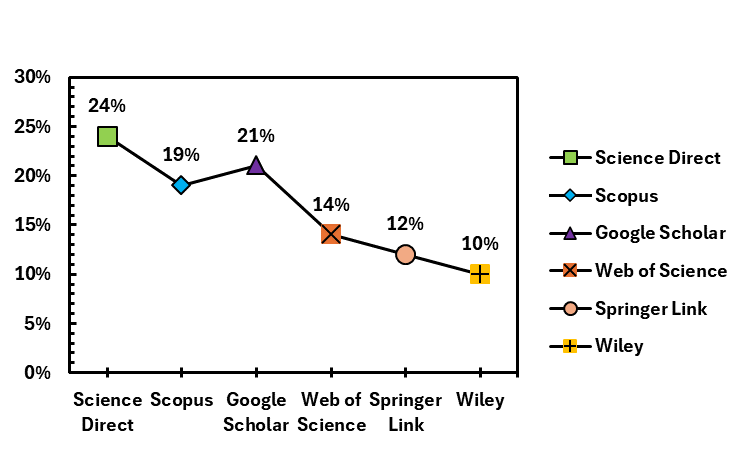
\includegraphics[width=\linewidth]{Percentages vs Database.png}
\caption{A Line Chart Illustrating the Distribution of the Selected Precision Agriculture Studies across Various Academic Databases (2021-2024)}
\label{fig}
\end{figure}

From Fig. 1, we see that Science Direct is referenced 24\% times, thus making it the most frequently used source. Scopus and Google Scholar are each used 19\% and 21\% times, respectively. This indicates their significant roles in our literature search. The Web of Science is utilized 14\% times, while Springer Link and Wiley are referenced 12\%, and 10\% times each, respectively. These distributions highlight the diverse range of databases we rely on to ensure a comprehensive review of the available literature.

The reliance on Science Direct and Google Scholar may bias the literature toward journals with broader international visibility, potentially underrepresenting region-specific case studies, highlighting the need for careful cross-region comparison.

\subsection{Scope and Time-Window Justification (2021–2024)}
We delimit our SLR to Jan 2021–Dec 2024 to capture the inflection point in Precision Agriculture where (i) transformer-based vision models and self/weakly supervised learning became practical, (ii) multimodal fusion of remote sensing (UAV/Sentinel) with in-field IoT and weather data matured, and (iii) explainable AI and interoperability began to appear in applied Precision Agriculture studies. Earlier reviews (2016–2020) provide broad coverage but predate these shifts, while very recent umbrella reviews (2024–2025) are not focused on yield-centric predictive workflows or cross-study comparability. Our novelty is a task-focused synthesis of 2021–2024 studies emphasizing data quality, multisource integration, interoperability, and external validation.

\subsection{Search Strategy}
We use a combination of keywords related to ML and DL algorithms in Precision Agriculture. The Boolean search strings included terms such as 
("precision agriculture" OR "smart farming" OR "digital agriculture") AND 
("machine learning" OR "deep learning" OR "transformer" OR "self-supervised") AND 
("yield" OR "irrigation" OR "disease" OR "soil" OR "remote sensing" OR "UAV" OR "Sentinel" OR "multimodal"). 
Searches were applied to titles, abstracts, and keywords. To reduce omissions, we also performed backward and forward snowballing on seed surveys published between 2021–2024. The literature retrieved includes journal articles, conference papers, and book chapters.

\subsection{Inclusion and Exclusion Criteria}
To involve relevant and quality studies, the following criteria are applied:

\begin{itemize}
\item \textbf{Inclusion Criteria:} The Precision Agriculture by either ML or DL algorithms, published in English and full text.
\item \textbf{Exclusion Criteria:} Studies not related to agriculture, review or survey papers, duplicate studies, and those published before 2021.
\end{itemize}

\begin{figure}[htbp]
\centering
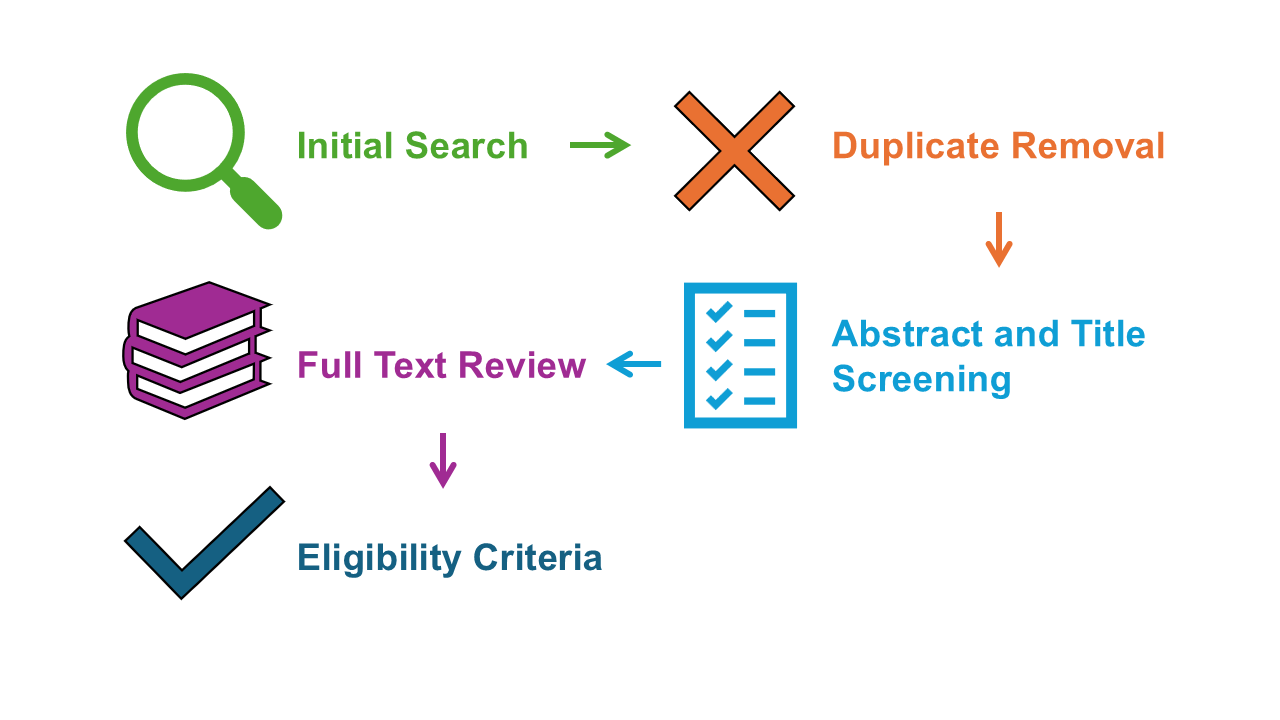
\includegraphics[width=\linewidth]{inex.png}
\caption{A Workflow Diagram Illustrating the Inclusion and Exclusion Criteria Used in the Selected Precision Agriculture Studies}
\label{fig}
\end{figure}

As shown in Fig. 3, the search initially returns 600 studies spanning from 2021 to 2024. After the removal of duplicate topics, there are 470 related studies. Abstract and title screening reduces the count to 230 studies. With the full-text review, the shortlist includes 140 studies. Finally, 100 studies are filtered for detailed analysis after applying the eligibility criteria. 

\begin{figure}[htbp]
\centering
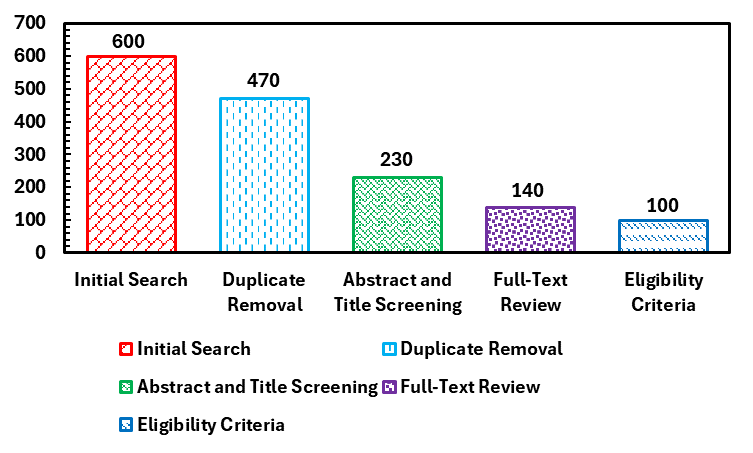
\includegraphics[width=\linewidth]{chart.png}
\caption{A Column Chart Illustrating the Inclusion and Exclusion Criteria Used in the Selected Precision Agriculture Studies}
\label{fig}
\end{figure}

Our SLR focuses on crop yield prediction and resource-allocation models. Weed/disease mapping papers (e.g., Rumex UAV+DL study, 2022) were excluded under this task filter, which we now state explicitly. 

\subsection{Study Selection}

The research studies spreading to all the continents in Fig. 4, suggest global significance. The research studies using ML and DL algorithms in Precision Agriculture are huge and diverse. After all, the highest share, which is 54\%, comes from Asia, which follows significant efforts taken to improve agricultural technologies in this region. 15\% of studies are available from North America. This shows their huge interest in applying advanced technologies to agriculture. About 11\% of the studies are from Europe. This indicates the active research background in Precision Agriculture on that continent. 10\% of the studies originate from Africa. It shows a growing regional emphasis on leveraging technology for improved agricultural productivity. 

\begin{figure}[htbp]
\centering
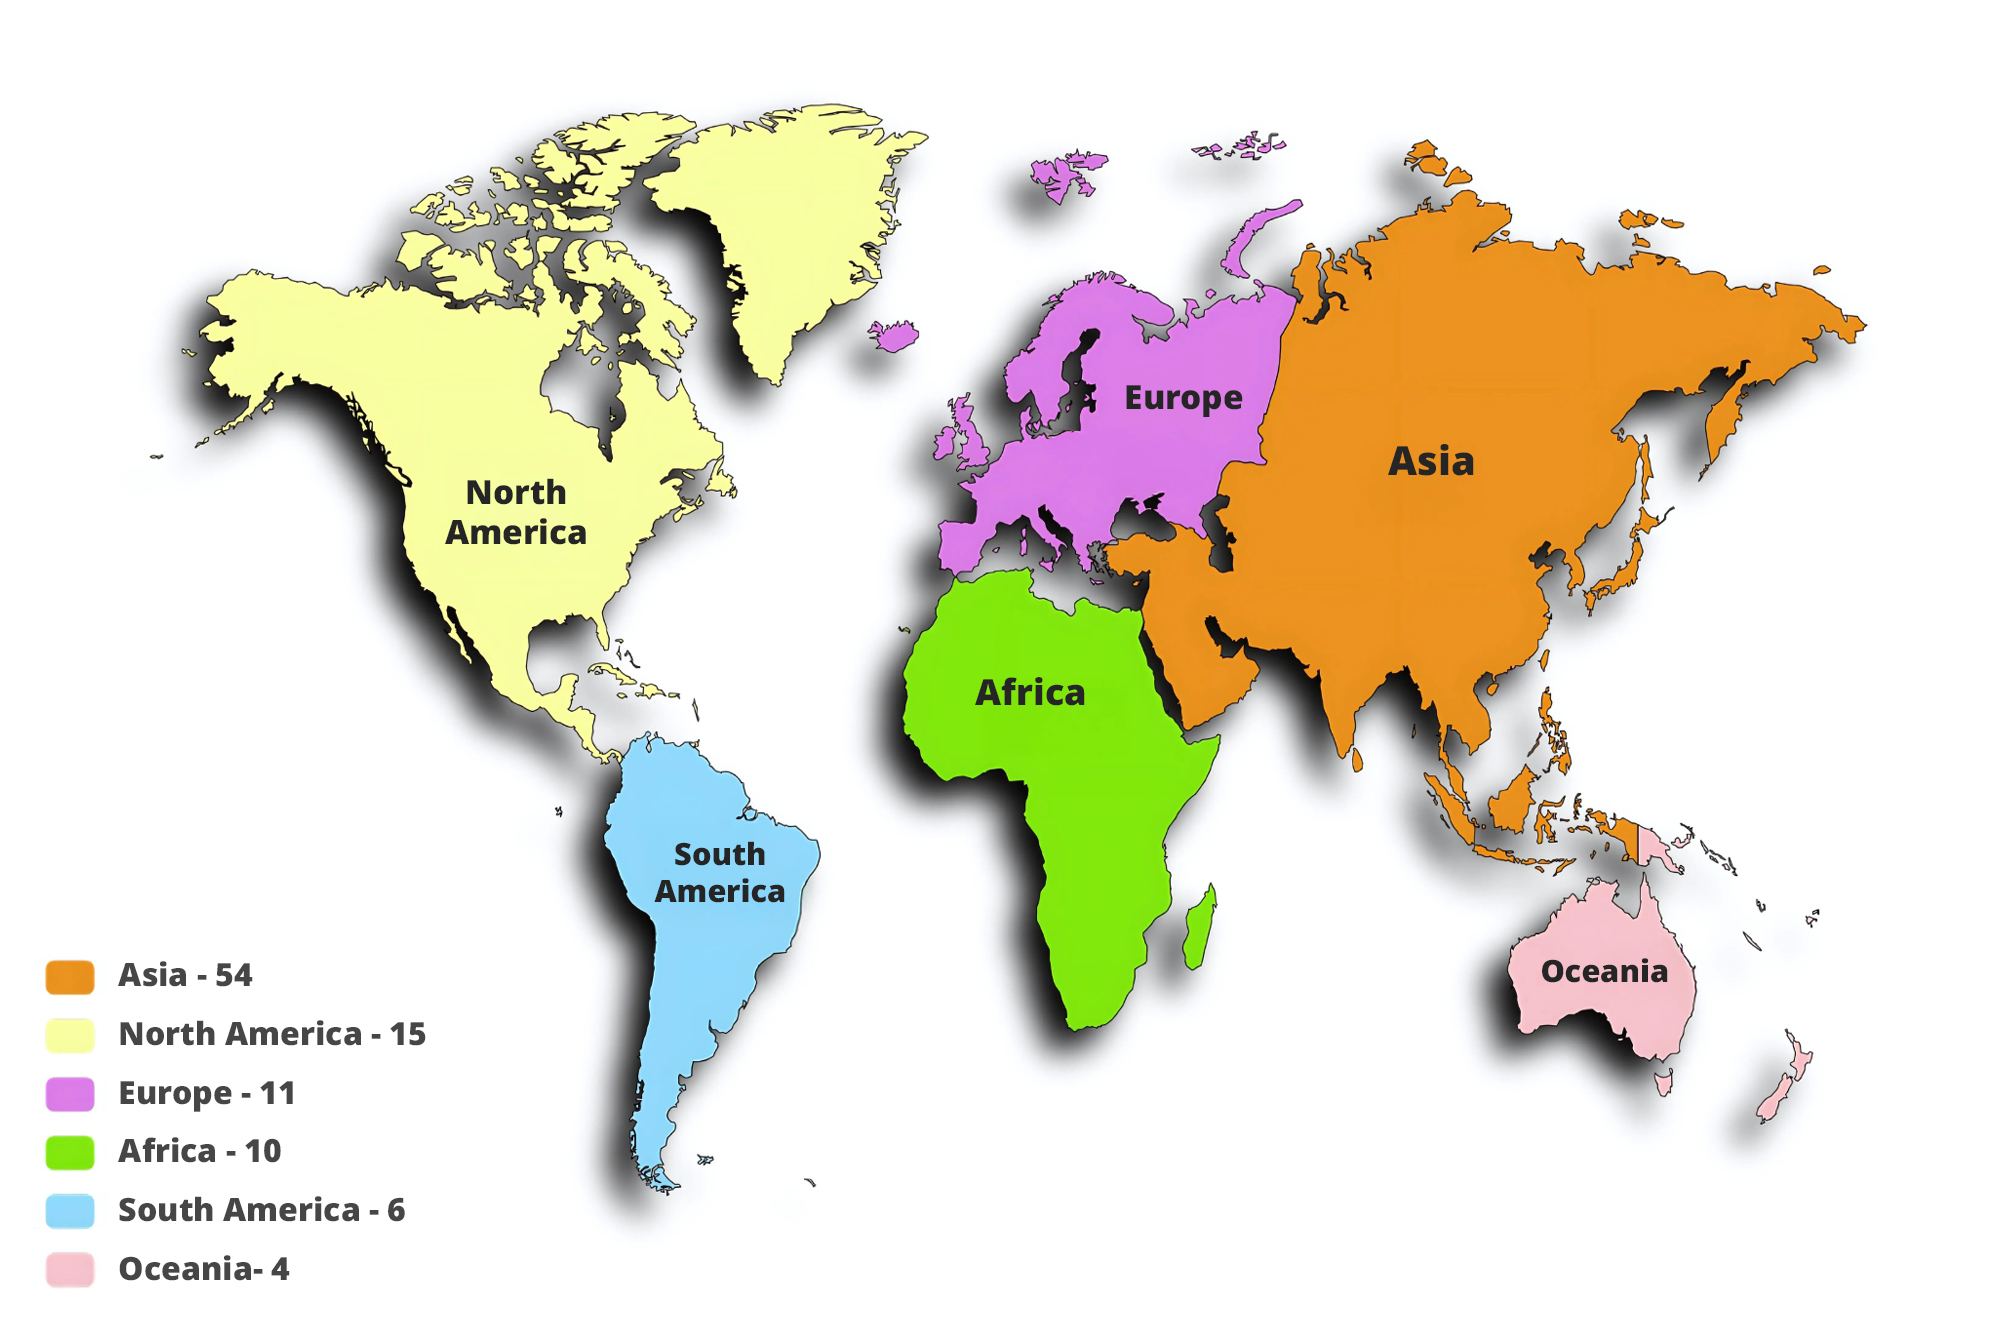
\includegraphics[width=\linewidth]{Map.jpg}
\caption{A Geo Chart Illustrating the Percentages of Selected Precision Agriculture Studies by Continent (2021-2024)}
\label{fig}
\end{figure}

South America, and Oceania contribute 6\%, and 4\% of the papers to this field, respectively, which indicates newly arrived interest. Therefore, this heterogeneity of study locations may underline the global relevance and the collaborative nature of efforts in improving methodologies for Precision Agriculture.

The predominance of studies from Asia (54\%) suggests that results are heavily influenced by region-specific cropping systems and climate conditions. Thus, model performance trends may differ in less-represented regions, emphasizing the need to assess the transferability of ML/DL approaches across geographies.

\subsection{Synthesis and Analysis}

We identify various uses of ML and DL algorithms in analyzing Precision Agriculture studies. The data flow diagram in Fig. 5, visualizes the process from data collection to prediction in Precision Agriculture. It also explicitly mentions the assistance of diverse data sources and algorithms.

\begin{figure}[htbp]
\centering
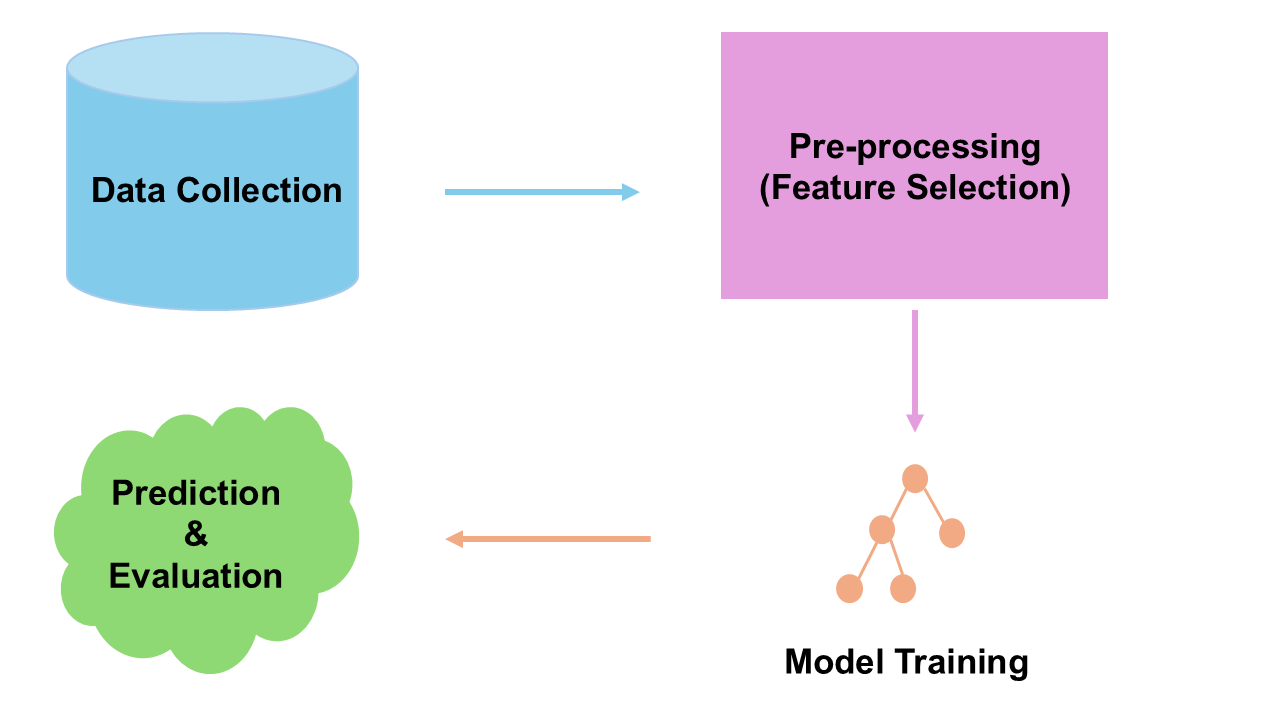
\includegraphics[width=\linewidth]{Data Flow Diagram.png}
\caption{A Data Flow Diagram Illustrating the Comprehensive Process Involved in Crop Yield Prediction in Precision Agriculture Using ML and DL Algorithms}
\label{fig}
\end{figure}

\begin{itemize}
\item \textbf{Data Collection:} It is acquiring data from satellite images, IoT sensors, soil sensors, and weather stations. These different data sources are important for accurately identifying variations in soil conditions, crop health, and environmental factors to ensure precise Crop Yield Prediction in Precision Agriculture.
\item \textbf{Pre-processing (Feature Selection):} The collected data goes through several pre-processing steps like cleaning data, normalization, feature extraction, and feature selection. These processes help eliminate noise, standardize formats, and isolate critical attributes, presenting data in a form that a model can be trained on to improve the prediction's accuracy. Data incompleteness or noise negatively affects the accuracy of SVM and linear models more than ensemble methods, which are more robust to missing or heterogeneous datasets. Scarce data particularly limits DL models, highlighting the importance of data augmentation or transfer learning strategies.
\item \textbf{Model Training:} The pre-processed data is then used to train ML and DL algorithms. In this phase, each algorithm learns patterns, relationships, and trends in the data that influence crop yields under specific conditions. Thus, it enables a robust and adaptable prediction mechanism.
\item \textbf{Prediction \& Evaluation:} This leads to a prediction of crop yields based on trained models. The results provide actionable insights that farmers and stakeholders can utilize for agricultural planning, optimizing resource usage, and making data-driven decisions to enhance productivity.
\end{itemize}

Studies are thematically grouped according to the applied algorithms of ML and DL, and evaluation metrics. We also find out which features are considered within these predictive models and the reported evaluation metrics. Then, the findings are synthesized. Finally, we look for common trends, strengths, and weaknesses in the current research landscape.

Heterogeneous datasets across regions (e.g., varying climate, soil type) show that model performance differs significantly by context. For example, models trained on irrigated wheat fields in North America may underperform on rainfed rice fields in Asia unless adapted via domain transfer techniques.

\begin{figure}[htbp]
\centering
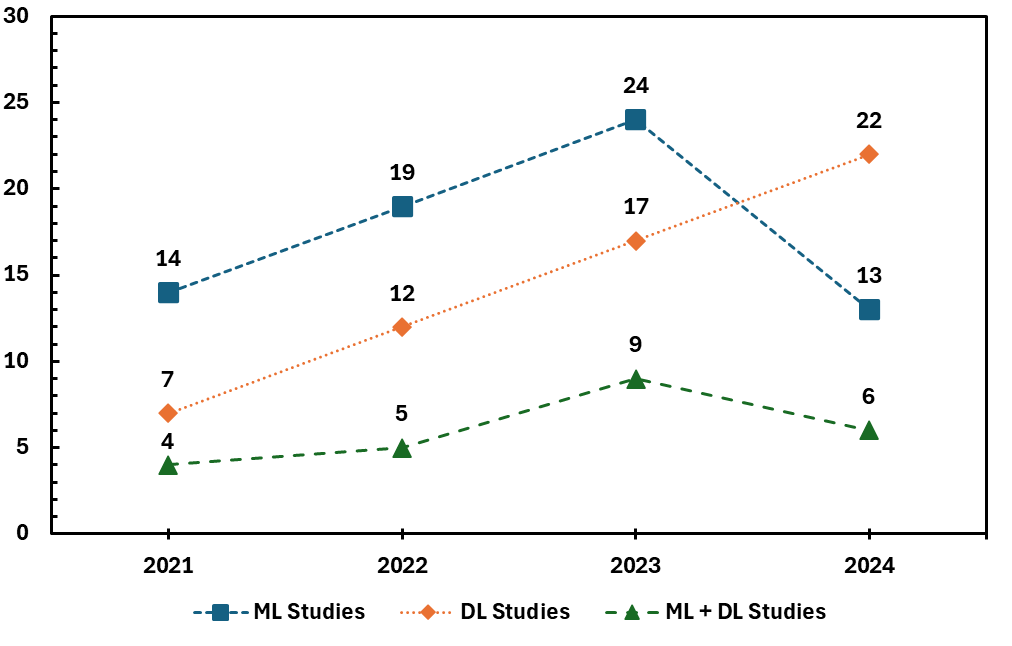
\includegraphics[width=\linewidth]{ML Papers and DL Papers.png}
\caption{A Line Chart Illustrating the Year-wise Distribution of ML and DL Algorithms Used in the Selected Precision Agriculture Studies (2021-2024)}
\label{fig}
\end{figure}

Although apparently, most of the research focus has moved from model development to Crop Yield Prediction in Precision Agriculture. Precision Agriculture using ML and DL algorithms has grown significantly from 2021 to 2024, as illustrated in Fig. 6. In 2021, our selected studies include 14 research studies on ML algorithms and 7 on DL algorithms. We find that with 4 studies utilizing both algorithms. This trend become more prominent in 2022. With the number of ML studies increasing to 19, DL studies to 12. And, 5 studies employing both algorithms can be seen. 

Continued growth is observed in 2023, with 24 studies on ML, 17 on DL, and 9 combining both. This highlights the rising interest and advancements in these algorithms. A significant shift occurs in 2024, with 21 DL studies surpassing 13 on ML and 6 studies integrating both algorithms. This distribution reflects the evolving research and innovation landscape in agricultural technology. Thus, it emphasizes the growing importance and application of advanced ML and DL algorithms in Precision Agriculture.

RF and GBM often outperform SVM and KNN in heterogeneous datasets due to their ability to handle non-linear relationships and missing values, making them suitable for regions with variable soil and weather data.

CNNs excel in integrating remote sensing imagery for spatial crop monitoring, whereas LSTMs are preferred for time-series prediction of yield or irrigation needs. DNNs provide flexibility but require large, high-quality datasets to avoid overfitting.

Models that integrate IoT, soil, and climate data consistently outperform those using only satellite imagery, demonstrating the critical impact of multisource and high-resolution data on predictive accuracy.

Across studies, RF and GBM models are consistently effective for cereal crops like wheat and maize, while CNNs perform better for crops requiring detailed canopy imagery such as rice or vegetables. Models evaluated under controlled greenhouse conditions often report higher accuracy than field trials, emphasizing the gap between lab-scale predictions and real-world applicability.

\subsection{Reporting}
Our review results are presented in the following sections. We comprehensively compare the ML and DL algorithms. We discuss the most significant features, and measure the evaluation metrics. Finally, we present major challenges and future Precision Agriculture research directions. 

This methodology ensures that the literature review is less biased and more systematic. It offers a well-rounded perspective. The insights drawn here aim to benefit researchers and practitioners working on Precision Agriculture. It guides them toward more effective strategies and innovative solutions.

Our analysis indicates that ensemble models and deep learning architectures perform best with integrated multi-modal data, while simpler models suffice for small or homogeneous datasets. Future work should prioritize addressing data scarcity, model transferability across regions, and explainability to improve adoption by practitioners.

\subsection{Key Terminologies and Prominent References}

Key terminologies and prominent references used in Precision Agriculture studies are systematically summarized in TABLE II \& III. These summaries serve as comprehensive guidelines to enhance the reader's understanding of this research area by covering essential ML and DL algorithms, evaluation metrics, and foundational concepts. ML and DL algorithms bring advanced analytical capabilities by transforming complex datasets into actionable insights that drive decision-making in agriculture.

Prominent references guide readers to foundational studies and recent advancements, providing a robust framework for further exploration. By reviewing these tables, readers can effortlessly navigate the specialized language and complex concepts, making sophisticated methodologies more accessible and applicable.

\begin{table*}[htbp]
\centering
\caption{Key Terminologies and their Overview in the Precision Agriculture Studies}
\begin{adjustbox}{width=\textwidth}
\begin{tabular}{|p{3cm}|p{4cm}|p{7cm}|}
\hline
\textbf{Category} & \textbf{Key Term} & \textbf{Overview} \\
\hline
Machine Learning (ML) Algorithms 
& Support Vector Machines (SVM) & A machine learning algorithm used to classify and regress data by finding the optimal hyperplane that separates data points of different classes. \\
\cline{2-3}
& Random Forests (RF) & An ensemble learning method that combines multiple decision trees to improve accuracy and robustness by reducing overfitting. \\
\cline{2-3}
& Gradient Boosting Machines (GBM) & An ensemble learning technique that improves Crop Yield Prediction by building models to correct errors made by previous models. \\
\cline{2-3}
& K-Nearest Neighbors (KNN) & An algorithm that classifies or predicts values based on the closest data points in the feature space. \\
\cline{2-3}
& Linear Regression (LR) & A statistical method that models the relationship between a dependent variable (crop yield) and independent variables (e.g., temperature, rainfall). \\
\cline{2-3}
& Decision Trees (DT) & A model that splits data into branches to make decisions and predict crop yields based on feature values. \\
\cline{2-3}
& Extreme Learning Machines (ELM) & A fast-learning algorithm for single-layer feedforward neural networks used to predict crop yields. \\
\cline{2-3}
& Bayesian Networks (BN) & A probabilistic graphical model representing variables and their conditional dependencies for crop yield prediction. \\
\cline{2-3}
& Naive Bayes (NB) & A probabilistic classifier that applies Bayes' theorem with strong independence assumptions between features. \\
\cline{2-3}
& Logistic Regression (LogR) & A statistical model used to predict binary outcomes in crop yield prediction. \\
\cline{2-3}
& Adaptive Neuro-Fuzzy Inference System (ANFIS) & A hybrid model combining neural networks and fuzzy logic to predict crop yields by learning and adapting to complex patterns in data. \\
\cline{2-3}
& Polynomial Regression (PR) & A regression technique used in crop yield prediction to model the relationship between input features and yield by fitting a polynomial equation. \\
\hline
Deep Learning (DL) Algorithms
& Artificial Neural Networks (ANN) & A deep learning model used to predict crop yields by learning complex patterns in agricultural data through interconnected layers of nodes. \\
\cline{2-3}
& Recurrent Neural Networks (RNN) & A type of neural network designed to recognize patterns in data sequences, making it suitable for predicting crop yields based on time-series data. \\
\cline{2-3}
& Convolutional Neural Networks (CNN) & Deep learning architecture used for image analysis in crop yield prediction, effectively capturing spatial features from remote sensing data. \\
\cline{2-3}
& Long Short-Term Memory (LSTM) & Recurrent neural network architecture designed to model temporal sequences in Crop Yield Prediction by capturing long-term dependencies. \\
\cline{2-3}
& Deep Neural Networks (DNN) & Complex models capable of learning intricate patterns in crop yield prediction data through multiple layers of abstraction and processing. \\
\hline
Evaluation Metrics & Root Mean Square Error (RMSE) & Provides the square root of the average squared differences between predicted and actual crop yields, measuring the standard deviation of prediction errors. \\
\cline{2-3}
& Mean Absolute Error (MAE) & Measures the average magnitude of errors between predicted and actual crop yields, offering a straightforward assessment of prediction accuracy. \\
\cline{2-3}
& Mean Squared Error (MSE) & Evaluates the average squared differences between predicted and actual crop yields, highlighting large prediction errors. \\
\cline{2-3}
& Mean Absolute Percentage Error (MAPE) & Measures the accuracy of crop yield predictions by expressing errors as a percentage of actual values. \\
\cline{2-3}
& R-squared (R²) & Indicates the proportion of variance in crop yield predictions explained by the model. \\
\cline{2-3}
& Coefficient of Determination (CD) & Measures the proportion of variance in crop yield explained by the model, indicating prediction accuracy. \\
\hline
\end{tabular}
\end{adjustbox}
\label{table:key_terms}
\end{table*}

\begin{table*}[htbp]
\centering
\caption{Early and Prominent References in the Precision Agriculture Studies}
\begin{adjustbox}{width=\textwidth}
\begin{tabular}{|p{2cm}|p{14cm}|}
\hline
\textbf{Key Terms} & \textbf{Early and Prominent Research References} \\
\hline
Precision Agriculture & McBratney, A., Whelan, B., Ancev, T. et al. Future Directions of Precision Agriculture. Precision Agric 6, 7–23 (2005). https://doi.org/10.1007/s11119-005-0681-8. \\
\hline
Crop Yield Prediction & J. A. Duke, "Crop Yield Prediction Using Historical Data and Simple Models," 1974. \\
\hline
ML Algorithms & P.Priya et al. “PREDICTING YIELD OF THE CROP USING MACHINE LEARNING ALGORITHM.” (2018).\\
\hline
SVM & S. Veenadhari, B. Misra and C. Singh, "Machine learning approach for forecasting crop yield based on climatic parameters," 2014 International Conference on Computer Communication and Informatics, Coimbatore, India, 2014, pp. 1-5, doi: 10.1109/ICCCI.2014.6921718.\\
\hline
RF & Jeong JH, Resop JP, Mueller ND, Fleisher DH, Yun K, Butler EE, et al. (2016) Random Forests for Global and Regional Crop Yield Predictions. PLoS ONE 11(6): e0156571. https://doi.org/10.1371/journal.pone.0156571. \\
\hline
GBM & Friedman, J.H. (2001). Greedy function approximation: A gradient boosting machine. Annals of Statistics, 29, 1189-1232. \\
\hline
KNN & Khan, H., Ghosh, S.M. (2020). Machine Learning Approach for Crop Yield Prediction Emphasis on K-Medoid Clustering and Preprocessing. In: Singh Tomar, G., Chaudhari, N.S., Barbosa, J.L.V., Aghwariya, M.K. (eds) International Conference on Intelligent Computing and Smart Communication 2019. Algorithms for Intelligent Systems. Springer, Singapore. https://doi.org/10.1007/978-981-15-0633-8-27.\\
\hline
LR & Khazaei, J., Naghavi, M. R., Jahansouz, M. R., Salimi-Khorshidi, G. (2008). Yield Estimation and Clustering of Chickpea Genotypes Using Soft Computing Techniques. Agronomy Journal, 100(4), 1077-1087. https://doi.org/10.2134/agronj2006.0244.\\
\hline
DT & Singh A, Ganapathysubramanian B, Singh AK, Sarkar S. Machine Learning for High-Throughput Stress Phenotyping in Plants. Trends Plant Sci. 2016 Feb;21(2):110-124. doi: 10.1016/j.tplants.2015.10.015. Epub 2015 Dec 1. PMID: 26651918.\\
\hline
ELM & S. Vashisht, P. Kumar and M. C. Trivedi, "Improvised Extreme Learning Machine for Crop Yield Prediction," 2022 3rd International Conference on Intelligent Engineering and Management (ICIEM), London, United Kingdom, 2022, pp. 754-757, doi: 10.1109/ICIEM54221.2022.9853054. \\
\hline
BN & Bi, C., Chen, G. (2011). Bayesian Networks Modeling for Crop Diseases. In: Li, D., Liu, Y., Chen, Y. (eds) Computer and Computing Technologies in Agriculture IV. CCTA 2010. IFIP Advances in Information and Communication Technology, vol 344. Springer, Berlin, Heidelberg. https://doi.org/10.1007/978-3-642-18333-1-37. \\
\hline
NB & Maazallahi, A., Thota, S., Kondaboina, N. P., Muktineni, V., Annem, D., Rokkam, A. S., Amini, M. H., Salari, M. A., Norouzzadeh, P., Snir, E., Rahmani, B. (2024). Na\"ive Bayes and Random Forest for Crop Yield Prediction. ArXiv. /abs/2404.15392. \\
\hline
LogR & Li, Y., Li, R., Ji, R., Wu, Y., Chen, J., Wu, M., Yang, J. (2024). Research on Factors Affecting Global Grain Legume Yield Based on Explainable Artificial Intelligence. Agriculture, 14(3), 438. https://doi.org/10.3390/agriculture14030438. \\
\hline
ANFIS & Khoshnevisan, B., Rafiee, S., Mousazadeh, H. (2013). Application of multi-layer adaptive neuro-fuzzy inference system for estimation of greenhouse strawberry yield. Measurement, 47, 903-910. https://doi.org/10.1016/j.measurement.2013.10.018. \\
\hline
PR & Kuradusenge, M., Hitimana, E., Hanyurwimfura, D., Rukundo, P., Mtonga, K., Mukasine, A., Uwitonze, C., Ngabonziza, J., Uwamahoro, A. (2022). Crop Yield Prediction Using Machine Learning Models: Case of Irish Potato and Maize. Agriculture, 13(1), 225. https://doi.org/10.3390/agriculture13010225. \\
\hline
DL Algorithms & Khaki, Saeed Wang, Lizhi. (2020). Crop Yield Prediction Using Deep Neural Networks. 10.1007/978-3-030-30967-1-13.\\
\hline
ANN & Hara, Patryk, Piekutowska, Magdalena, Niedbała, Gniewko. (2021). Selection of Independent Variables for Crop Yield Prediction Using Artificial Neural Network Models with Remote Sensing Data. Land. 10. 609. 10.3390/land10060609. \\
\hline
RNN & Khaki S, Wang L, Archontoulis SV. A CNN-RNN Framework for Crop Yield Prediction. Front Plant Sci. 2020 Jan 24;10:1750. doi: 10.3389/fpls.2019.01750. PMID: 32038699; PMCID: PMC6993602.\\
\hline
CNN & Srivastava, A.K., Safaei, N., Khaki, S. et al. Winter wheat yield prediction using convolutional neural networks from environmental and phenological data. Sci Rep 12, 3215 (2022). https://doi.org/10.1038/s41598-022-06249-w. \\
\hline
LSTM & Kumar, V. Ramesh, K. Rakesh, V.. (2023). Optimizing LSTM and Bi‑LSTM models for crop yield prediction and comparison of their performance with traditional machine learning techniques. Applied Intelligence. 10.1007/s10489-023-05005-5. \\
\hline
DNN & Khaki S, Wang L. Crop Yield Prediction Using Deep Neural Networks. Front Plant Sci. 2019 May 22;10:621. doi: 10.3389/fpls.2019.00621. PMID: 31191564; PMCID: PMC6540942. \\
\hline
RMSE & Kaul, M., Hill, R. L., Walthall, C. (2005). Artificial neural networks for corn and soybean yield prediction. Agricultural Systems, 85(1), 1-18. https://doi.org/10.1016/j.agsy.2004.07.009. \\
\hline
MAE & Sánchez, Alberto González et al. “Predictive ability of machine learning methods for massive crop yield prediction.” Spanish Journal of Agricultural Research (2014): 313-328. \\
\hline
MSE & Everingham, Y., Smyth, C., Inman-Bamber, N. (2009). Ensemble data mining approaches to forecast regional sugarcane crop production. Agricultural and Forest Meteorology, 149(3-4), 689-696. https://doi.org/10.1016/j.agrformet.2008.10.018. \\
\hline
MAPE & Bolton, D. K., Friedl, M. A. (2013). Forecasting crop yield using remotely sensed vegetation indices and crop phenology metrics. Agricultural and Forest Meteorology, 173, 74-84. https://doi.org/10.1016/j.agrformet.2013.01.007. \\
\hline
R² & M. G. Ananthara, T. Arunkumar and R. Hemavathy, "CRY — An improved crop yield prediction model using bee hive clustering approach for agricultural data sets," 2013 International Conference on Pattern Recognition, Informatics and Mobile Engineering, Salem, India, 2013, pp. 473-478, doi: 10.1109/ICPRIME.2013.6496717.\\
\hline
CD & Kuradusenge, M.; Hitimana, E.; Hanyurwimfura, D.; Rukundo, P.; Mtonga, K.; Mukasine, A.; Uwitonze, C.; Ngabonziza, J.; Uwamahoro, A. Crop Yield Prediction Using Machine Learning Models: Case of Irish Potato and Maize. Agriculture 2023, 13, 225. https://doi.org/10.3390/agriculture13010225. \\
\hline
\end{tabular}
\end{adjustbox}
\label{table:key_terms}
\end{table*}

Important features such as IoT devices, weather data, soil information, remote sensing, climate data, and disease detection are meticulously included later on. They play a pivotal role by enabling real-time data collection through sensors deployed in the field, monitoring factors like soil moisture, temperature, and crop health continuously. This integration facilitates precise irrigation, fertilization, and pest management, directly influencing crop yield and overall productivity.

Weather data, including temperature, rainfall, and solar radiation, significantly impact crop health and yield. Soil information, such as moisture levels and nutrient content directly affects plant growth and productivity. Remote sensing, utilizing satellite imagery, offers a bird's-eye view of crop growth and health patterns, allowing for large-scale monitoring and timely interventions. Additionally, disease detection through image analysis and sensor data helps in the early identification and management of crop diseases, preventing yield losses and ensuring sustainable agricultural practices.

Climate data contextualizes broader environmental effects, helping in understanding long-term trends and their implications on agriculture. The incorporation of satellite images enhances the accuracy of monitoring and supports the analysis of spatial and temporal variations in crop conditions.

\section{Review of ML and DL Algorithms used in the Selected Precision Agriculture Studies}

We have identified the most used ML and DL algorithms applied to Precision Agriculture during the analysis. From our analysis, the following ML algorithms are the most frequently used: 

\begin{itemize}
\item SVM
\item RF
\item GBM
\item KNN
\item LR
\item DT
\item ELM
\item BN
\item NB
\item LogR
\item ANFIS
\item PR
\end{itemize}

Let us thoroughly review these algorithms and summarize them (TABLE IV) for a better understanding.

% table
\begin{table*}[htbp]
\centering
\caption{Overview of Key Aspects in Some Recently Selected Precision Agriculture Studies}
\begin{adjustbox}{width=\textwidth}
\begin{tabular}{|p{3cm}|p{1cm}|p{3cm}|p{3cm}|p{3cm}|p{1cm}|p{2cm}|}
\hline
\textbf{Authors} & \textbf{Year} & \textbf{Application Domains} & \textbf{Features} & \textbf{Algorithms/Techniques} & \textbf{Country} & \textbf{Crop}\\
\hline
Rachid Ed-Daoudi et al. & 2023 & Crop Yield Analysis & Weather Patterns, Soil Moisture, Rainfall & RF, Neural Networks & Morocco & Not Specified \\
\hline
Y. Wang, W. Shi, T. Wen & 2023 & Optimal Water and Nitrogen Application & Soil Moisture, Temperature, Rainfall & Gaussian Process Regression & China  & Winter Wheat\\
\hline
SANJANA M & 2023 & General Crop Yield Prediction & Soil Type, Temperature, Rainfall & Data Mining, ICT Methods & India & Rice \\
\hline
Arpitha Varghese, Mamatha Inna & 2023 & Unified Crop Recommendation System & Soil and Environmental Data & ML and IoT & India & Not Specified\\
\hline
Shinde Shivnanda et al. & 2023 & Smart Farming Yield Prediction & Soil Moisture, Rainfall & RF & India & Not Specified\\
\hline
Ahmadfaraz Ishaq et al. & 2023 & Systematic Radiative Transfer Review & Soil Type, Leaf Area Index, Chlorophyll & PROSAIL & China & Not Specified\\
\hline
Moon Halder et al. & 2023 & ML-Based Yield Prediction Review & Temperature, Rainfall & ML Algorithms (Various) & Global & Not Specified\\
\hline
Prof. Dr. Komati Satish & 2023 & GELM-Based Yield Prediction & Soil Factors & Gaussian Extreme Learning Machine (GELM) & India & Not Specified\\
\hline
Mildred Virginia López Segura et al. & 2023 & XGBoost Yield Prediction & Pruning, Cleaning, Pest Control, Weather Elements & XGBoost & Mexico & Persian Lemon\\
\hline
Vijayatai Hukare et al. & 2023 & Crop Yield Prediction Methods & Soil Type, Climate Parameters & Gradient Boosting Regression & India & Sugarcane\\
\hline
Jayshree Hajgude, Tanuja Sarode & 2023 & Comparative Ensemble Models Study & Temperature, Rainfall & AdaBoost Regressors & India & Soybean\\
\hline
Qi Zhang et al. & 2023 & Variety Yield Data Compensation & Temperature, Soil Moisture & CVYPS-VYDC & China & Maize \\
\hline
S. Archana, Senthil Kumar & 2023 & Deep Learning-Based Yield Prediction & Temperature, Rainfall & LSTM, DL Methods & India & Not Specified\\
\hline
Venkata Rama Rao Kolipaka et al. & 2023 & Temporal Yield Prediction Fluctuations & Rainfall, Temperature & LSTM, CNN & India & Not Specified\\
\hline
Seyed Erfan Momenpour et al. & 2024 & Bibliometric Yield Prediction Analysis & Literature Review & Various & Iran & Not Specified\\
\hline
Dr Kavita Jhajharia, Pratistha Mathur & 2024 & Regional Yield Prediction & Rainfall, Soil Type & RF, Gradient Boosting & India & Not Specified\\
\hline
Subramanian Shanmuga Priya et al. & 2023 & Soybean Yield Prediction & Rainfall, Soil Type & LSTM & USA & Soybean\\
\hline
Yuchi Ma et al. & 2023 & Deep Learning Domain Adaptation & Temperature, Soil Moisture & Partial Domain Adversarial Neural Network (PDANN) & USA & Corn and Soybean\\
\hline
Shevanthe Sekar, Sathiyamoorthy E & 2023 & Systematic ML Study & Rainfall, Temperature & RF & Global & Not Specified\\
\hline
Venkata Rama Rao Kolipaka et al. & 2024 & Hybrid Yield Prediction & Rainfall, Temperature & Deep Belief Networks, LSTM, CNN & India & Not Specified\\
\hline
Benjamin Kwapong Osibo et al. & 2023 & Hybrid Yield Prediction & Soil Data, MODIS Data, Climatic Variables & LSTM, XGBoost & Canada & Not Specified\\
\hline
Rajneesh Kumar et al. & 2024 & XGBoost Yield Prediction & Soil, Environmental Data & XGBoost, 1D-CGRU & India & Not Specified\\
\hline
Toshihiro Sakamoto et al. & 2023 & Crop Monitoring System & Crop Phenology, Crop Classification & Multiple Algorithms (including MODIS) & USA & Corn and Soybeans\\
\hline
Swanth Boppudi, Sheela J et al. & 2024 & Deep Ensemble Model Yield Prediction & Higher-order Features, Enhanced Entropy-based Features & CNN, Bi-GRU, IBS-BOA & India & Not Specified\\
\hline
Benjamin Kwapong Osibo et al. & 2024 & Hybrid Yield Prediction & Soil Data, MODIS Data, Climatic Variables & LSTM, XGBoost & Canada & Not Specified\\
\hline
\end{tabular}
\end{adjustbox}
\label{table:summary}
\end{table*}

\subsection{SVM}\label{AA}
SVMs work well on high-dimensional data. They perform elegantly with small to medium-sized datasets. And they are robust in distinguishing separate classes within given data \cite{b11}. SVMs use kernel functions to 'trick' the data into avoiding this curse. 

However, this pioneer's inseparable relationship with kernel choice and hyperparameters can make it hard to choose correctly. Not to mention computationally burdensome. They may also be less effective with very large data. For example, on average, the higher accuracy (92\%) for an SVM model trained on a dataset with 5,000 samples drops significantly to 78\% when applied to a dataset of 50,000 samples with no proper kernel tuning \cite{b12}.

\subsection{RF}\label{AA}
RFs are robust, easy to use, and less prone to overfitting than individual decision trees. They can take large, high-dimensional datasets by making several decision trees and merging their results.

At the same time, RF is computationally very expensive for large data sets and has very limited interpretability due to the complexity of the ensemble of trees \cite{b13}. RF models may not show their best capacity with large, noisy data. We find that, on average RF models have an accuracy of 85\% if the data used is clean and falls down to 70\% using noisy data \cite{b14}.

\subsection{GBM}\label{AA}
GBM combines the strengths of several weak learners with the capability to fashion prediction accuracy. It builds the model sequentially, correcting errors made by the previous model \cite{b15}. 

GBMs take quite a long time to train, and their hyperparameters need proper tuning in balance to avoid overfitting. Due to their complexity, they are rather hard to interpret and computationally demanding, especially in large datasets. While training on 100,000 samples takes on average 10 hours for a GBM model, it takes only 1 hour for some simple models like LR \cite{b16}. 

\subsection{KNN}\label{AA}
KNN is a very simple yet effective algorithm that works well when the feature space is well-defined, and the dataset is limited. The concept of this classifier is to classify data using the closest training examples in the feature space \cite{b17}. 

Nevertheless, performance may degrade for large datasets because finding the nearest neighbors computationally has a higher cost. It is also sensitive to the choice of distance metric and the number of neighbors (k). Due to the curse of dimensionality, it performs poorly in high-dimensional spaces. On average, we find that KNN performs an accuracy of 90\% on low-dimensional data. But on a high-dimensional dataset, the accuracy drops to 60\% \cite{b18}. 

\subsection{LR}\label{AA}
LR is simple, very interpretable, and has been in large-scale use for Precision Agriculture. This models the relationship between the independent variable, crop yield, and one or more independent variables—or features—with a fitting of the linear equation \cite{b19}. 

Still, LR presumes linearity between variables. While it is sensitive to outliers, this may not always be the case. And hence performs poorly on nonlinear data. LR can perform well in simple, linear relationships but fails in complex, nonlinear patterns. Our findings establish that, on average LR has an accuracy level of only 50\% on nonlinear data as opposed to 80\% on linear data \cite{b20}.

\subsection{DT}\label{AA}
DTs are intuitive, easy to interpret, and powerful in handling numerical and categorical data. They recursively split the data into subsets according to the value of input features. 

Nonetheless, DTs are prone to overfitting. Especially when the tree is too complex, and sensitive to small changes in data \cite{b21}. DTs work well on low-dimensional but poorly on high-dimensional datasets. On average DTs give an accuracy of 85\% using a dataset that contained 10 features and falls to 60\% utilizing a dataset that contained 100 features \cite{b22}. This decline is often attributed to the model's increased complexity and the risk of overfitting. Mainly when dealing with a high-dimensional feature space.

\subsection{ELM}\label{AA}
ELMs will display fast learning speed with good generalization performance. They are a Feedforward Neural Network (FNN) with only a single hidden layer.

Conversely, it has been documented that ELMs can still be very sensitive to the number of hidden neurons and the selection of input weights and biases \cite{b23}. Their performance varies significantly when configured differently. According to our study, on average the accuracy achieved for the optimum configuration is 80\%, while it is as low as 55\% with suboptimum configuration \cite{b24}.

\subsection{BN}\label{AA}
BNs reduce uncertainty and embed domain knowledge into the model. A probabilistic graphical model represents the conditional dependencies between variables \cite{b25}. 

Yet, BNs are computationally time-consuming. Particularly for large and complex datasets that require much insight into the underlying dependencies of variables. According to our findings, on average BNs have an accuracy of 75\% when domain knowledge is well integrated. But it drops to 50\% where the dependencies are not well understood \cite{b26}. 

\subsection{NB}\label{AA}
NB is simple, efficient, and effective in accomplishing some Precision Agriculture tasks. As a Bayesian probabilistic classifier based on Bayes' theorem, it assumes independence between the features \cite{b27}. 

Regardless, in most cases, the feature independence assumption is unrealistic. Therefore, it limits NB's accuracy and requires huge training datasets for good performance. According to our studies, on average NB achieves 66\% accuracy for large datasets but only 40\% accuracy for small sets of data. This is likely due to the reduced amount of data leading to less reliable probabilistic predictions \cite{b28}. 

\subsection{LogR}\label{AA}
LogR returns the probability of a given event occurring. It is a logistic regression for binary tasks. It models the probability of the target variable's expression as a logistic function of input features. 

Anyhow, LogR assumes linearity in the relationship between input features and log odds of the target variable. Thus, on a non-linear dataset, it may not perform well. Using the same data set, on average LogR reaches an accuracy of 70\% when the data is linear and only 50\% when it is nonlinear \cite{b29}. It reflects the algorithm's limitations in handling complex, non-linear relationships without transformations or advanced techniques.

\subsection{ANFIS}\label{AA}
ANFIS integrates neural networks and fuzzy logic to deal with uncertainty and approximate nonlinear relationships. hence, it acquires the benefits of both in Precision Agriculture. 

Despite this, the ANFIS model can turn out to be computationally intensive. And, it may have some parameter-tuning problems. Whereby the presence of both neural networks and fuzzy logic makes the model difficult to understand. With optimal tuning, on average ANFIS achieves an accuracy of 80\%, but with suboptimal tuning, ANFIS manages to attain an accuracy of 55\% \cite{b30}.

\subsection{PR}\label{AA}
PR is a generalization of LR. Whereby it uses a polynomial equation to fit the data, which models nonlinear relationships and complex patterns against LR \cite{b31}. 

On the other hand, PR models can become too complicated when including high-degree polynomials, suffering from overfitting. So, the polynomial degree should be chosen carefully to trade off model complexity with performance \cite{b32}. 

In recent years, DL algorithms have dominated Precision Agriculture since they can model complex patterns and relations within large datasets. DL algorithms commonly used in the analyzed studies include the following:

\begin{itemize}
\item ANN
\item RNN
\item CNN
\item LSTM
\item DNN
\end{itemize}

Now, a full review of these DL algorithms used in Precision Agriculture is detailed below.

\subsection{ANN}\label{AA}
ANNs are especially fitting to model complicated and nonlinear relationships between the input features and crop yields. This makes them unique in modelling complex patterns in a big dataset \cite{b33}. They depend on temperature, rainfall, and soil type inputs, among other features, for Precision Agriculture. 

However, the major problem is over-sizing, especially on small and noisy datasets. The model will learn the training data too well, plus its noise and outliers. ANN requires huge computational resources and expertise in tuning hyperparameters for optimal performance. Their "black-box" nature makes them difficult to interpret. We find that on average on a huge dataset like 10,000 samples, ANNs predict crop yields with an accuracy of 90\% \cite{b34}. Whereas, on average on smaller datasets like 1,000 samples, it drops to merely 75\% \cite{b35}.

\subsection{RNN}\label{AA}
RNNs are mainly designed for sequence prediction tasks. They are seamlessly effective for time series data. They capture temporal dependencies of data. Hence, it holds great potential for Precision Agriculture based on historical weather and climate data \cite{b36}. 

After all, RNNs may suffer from the problem of vanishing or exploding gradients. The training becomes difficult. Also, large amounts of data and computational resources are required. On average, we find that RNNs can be as accurate as 85\% in cases with extended data. But in those cases, with limited data, it drops to 60\% \cite{b37}. This decline highlights the importance of having big data for training complex algorithms like RNNs. This relies heavily on sequential data patterns to make accurate predictions.

\subsection{CNN}\label{AA}
CNNs are an appropriate choice in analyzing spatial data and images, such as satellite or UAV imagery used in crop monitoring. It has successfully captured hierarchical patterns and features in images for Precision Agriculture using visual data \cite{b38}.

Despite that, CNNs require large datasets and medium to high-range computational resources to train. As a result, this complexity in architecture may make them hard to interpret and have bad performance with limited or low-quality data. Moreover, tuning the hyperparameters and designing the network architecture is challenging and time-consuming.

\subsection{LSTM}\label{AA}
LSTMs are another class of RNNs that can overcome classical RNNs in handling long-term dependencies embedded in sequential data. LSTMs have proven helpful in time-series prediction tasks. Therefore, it is also used in Precision Agriculture based on weather and climate data \cite{b39}. LSTM networks can learn trends and seasonality in climate and crop growth data. This is efficient enough to permit Crop Yield Prediction with a high degree of accuracy, on average ranging from 75\% to 90\% depending on the specific dataset and the configuration used \cite{b40}.

Most of them are computationally time-intensive and usually require a really huge amount of data for training. It is complex to train and tune and might suffer from issues like vanishing or exploding gradients. Furthermore, it has very limited interpretability due to the intricate architecture of an LSTM model.

\subsection{DNN}\label{AA}
DNN represents a class of neural networks containing many hidden layers. It enables modelling complex and nonlinear relationships in data \cite{b41}. They have been employed to precision agriculture tasks successfully in several applications. This becomes possible as this algorithm may learn over large datasets and capture intricate patterns. DNN predicts crop yields at high accuracy levels, on average around 85\% - 90\%, by fusing weather conditions, soil types, and crop management practices \cite{b42}.

DNNs may suffer from overfitting, especially with small datasets. They require massive computational resources and expertise in hyperparameter tuning. Their black-box nature makes them very difficult to interpret. This generally restricts our understanding of the precise factors underlying the predictions.

From Fig. 7, we can see that ANN is used by 26.3\% of the studies that we have reviewed. This supports that the algorithm is famous and effective for this research area. Next in line is SVM with 18.1\%. This shows the strength of this algorithm in conducting classification and regression tasks.

\begin{figure}[htbp]
\centering
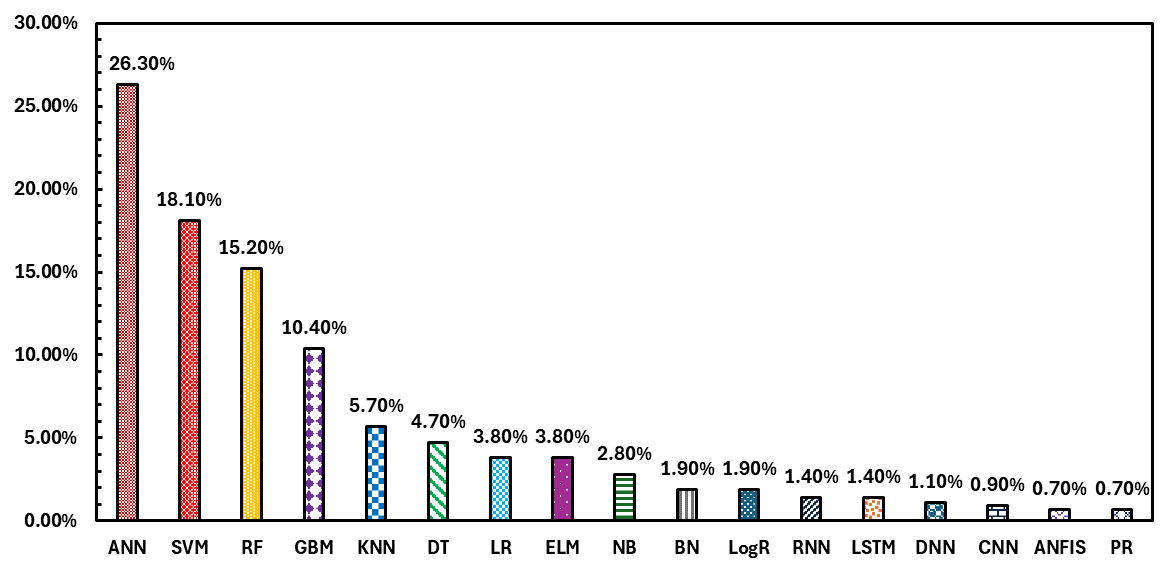
\includegraphics[width=\linewidth]{Percentage Distribution.png}
\caption{A Column Chart Illustrating the Distribution of ML and DL Algorithms Used in the Selected Precision Agriculture Studies (2021-2024)}
\label{fig}
\end{figure}

Next in line, RF accounts for 15.2\%. This reflects its capability to handle large datasets with high dimensionality. Compared with GBM in 10.4\% of the studies, where efficiency in predictive performance enhancement is shown. KNN, LR, and DT each contribute 5.7\%, 3.8\%, and 4.7\%, respectively. They act as a foundation for ML applications. ELM indicates 3.8\% of the studies. BN and NB are found in 1.9\% and 2.8\% studies. Therefore, it occupies a place in some limited and specific spheres of applications. Finally, LogR, RNN, CNN, LSTM, DNN, ANFIS, and PR each account for 1.9\%, 1.4\%, 0.9\%, 1.4\%, 1.1\%, 0.7\%, 0.7\% of studies. Thus, showing their emerging use and niche applications in Precision Agriculture research.

It is important to understand the significance of accurate Crop Yield Prediction in agricultural planning and decision-making. And how the integration of ML and DL algorithms has revolutionized these predictions by analyzing vast datasets, including weather patterns, soil types, and historical yield data. These advanced algorithms can identify complex patterns and trends. Thus, leading to more precise and reliable yield predictions. As a result, stakeholders can make better-informed decisions, optimize resource allocation, and improve food security.

\begin{figure}[htbp]
\centering
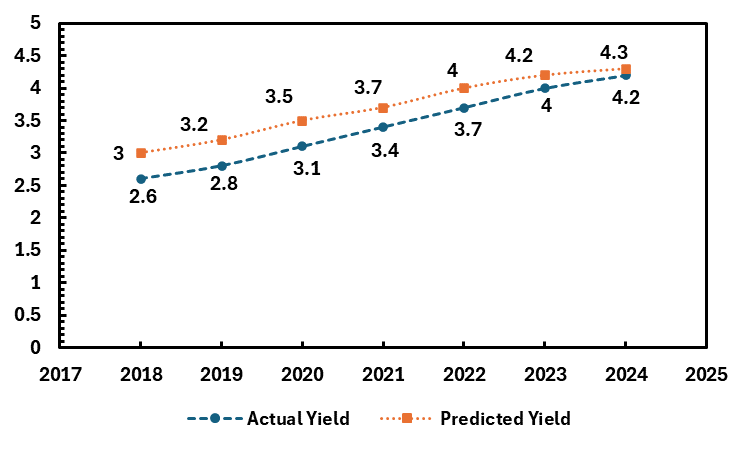
\includegraphics[width=\linewidth]{Predicted Yield and Actual Yield.png}
\caption{A Line Graph Illustrating the Predicted vs. Actual Crop Yields from 2018 to 2024 (Wheat Yields in India)}

\label{fig}
\end{figure}

Fig. 8 is the line graph indicating the predicted and actual wheat yields in India starting from 2018 up to 2024 \cite{b43}. This trend analysis shows predicting wheat yields in India over the years, reflecting the growing importance of Precision Agriculture. From the data provided, we can rightly conclude that Crop Yield Prediction in Precision Agriculture has increased in accuracy over the years. For instance, 2018 has a prediction of 3.0 tons per hectare against an actual yield that turned out slightly less at 2.6 tons per hectare. In 2019, the projected yield of 3.2 tons per hectare also stands close to 2.8 tons per hectare. In 2020, the projected yield of 3.5 tons per hectare is slightly higher than that of 3.1 tons per hectare. For 2021 and 2022, the projected yields are 3.7 and 4.0 tons per hectare, respectively. This is not very far from the actual yields, reaching 3.4 and 3.7 tons per hectare, respectively. Finally, in 2024, it is predicted that the projected yield will be very near the actual yield level at 4.3 and 4.2 tons per hectare, respectively.

In 2018-19, the more significant gap between predicted and actual yields (0.4 tons/hectare) reflects the early stages of applying ML and DL algorithms. When the models may not fully capture all the variables influencing yield, as more data becomes available and models are fine-tuned in 2020-22, the gap decreases to 0.3 tons/hectare, which shows improved accuracy in predictions. With further advancements in ML and DL algorithms and better integration of data sources, the gap narrows further to 0.2 and then 0.1 tons/hectare in 2023-24. This indicates highly reliable Crop Yield Predictions that closely match the actual yields.

This trend analysis indicates that the applied ML and DL algorithms are increasingly precise and reliable. Thus, it has proven effective in Precision Agriculture and may help in agricultural planning. By analyzing trends in actual and predicted yields, we can evaluate the effectiveness of current agricultural practices and technological interventions.

\begin{figure*}[htbp]
\centering
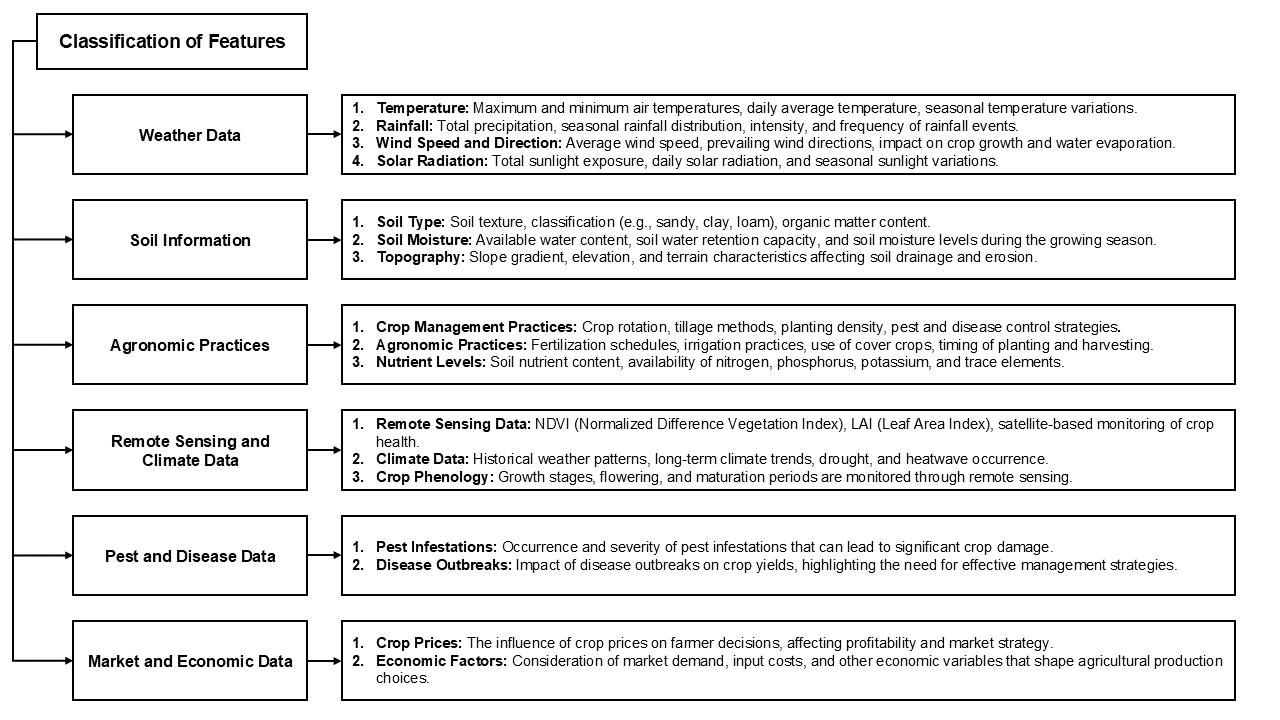
\includegraphics[width=\textwidth]{Tree.png}
\caption{A Hierarchical Classification of Features Used in the Selected Precision Agriculture Studies, Organized by Categories Such as Weather Data, Soil Information, Agronomic Practices, Remote Sensing and Climate Data, Pest and Disease Data, and Market and Economic Data}

\label{fig}
\end{figure*}

\section{Features and Data Used in the Selected Precision Agriculture Studies}

In a nutshell, for Precision Agriculture, the accuracy is mainly based on the quality and relevance of the input features. According to our analysis of 100 studies, the following features are the most used ones:

\begin{itemize}
\item Temperature
\item Rainfall
\item Soil Type
\item Crop Management Practices
\item Remote Sensing Data
\item Climate Data
\item Soil Moisture
\item Crop Phenology
\item Pest and Disease Incidence
\item Nutrient Levels
\item Topography
\item Solar Radiation
\item Wind Speed and Direction
\item Agronomic Practices
\item Market and Economic Data
\end{itemize}

\begin{table*}[t]
\centering
\caption{Summary of Features Utilized in Some Recently Selected Precision Agriculture Studies}
\label{table:features_summary}
\begin{adjustbox}{max width=\textwidth}
\begin{tabularx}{\textwidth}{|p{3cm}|p{3cm}|X|X|X|X|X|X|X|X|}
\hline
\textbf{Authors} & \textbf{Data Set} & \textbf{Temp.} & \textbf{Rainfall} & \textbf{Soil Type} & \textbf{Crop Mgmt.} & \textbf{Remote Sensing Data} & \textbf{Climate Data} & \textbf{Soil Moisture} & \textbf{Crop Phenology} \\
\hline
Rachid Ed-Daoudi (2023) & Crop Data, Morocco & \ding{51} & \ding{51} & \ding{51} & & \ding{51} & \ding{51} & & \\
\hline
Y. Wang, W. Shi, T. Wen (2023) & Wheat yield data, North China Plain & \ding{51} & \ding{51} & & & & \ding{51} & & \\
\hline
SANJANA M (2023) & Crop yield data, India & \ding{51} & \ding{51} & \ding{51} & & & & & \\
\hline
Arpitha Varghese, Mamatha Inna (2023) & IoT-based crop data, India & \ding{51} & & \ding{51} & \ding{51} & & \ding{51} & & \\
\hline
Shinde Shivnanda (2023) & Smart farming data, India & \ding{51} & \ding{51} & & \ding{51} & & & \ding{51} & \\
\hline
Ahmadfaraz Ishaq (2023) & Systematic review data, China & & \ding{51} & \ding{51} & & \ding{51} & \ding{51} & & \\
\hline
Moon Halder (2023) & Systematic review data, Bangladesh & \ding{51} & \ding{51} & & \ding{51} & & \ding{51} & & \\
\hline
Prof. Dr. Komati Satish (2023) & GELM-based yield data, India & & \ding{51} & \ding{51} & \ding{51} & & \ding{51} & \ding{51} & \\
\hline
Mildred Virginia López Segura (2023) & Persian lemon data, Mexico & & \ding{51} & & \ding{51} & & \ding{51} & & \\
\hline
Vijayatai Hukare (2023) & Sugarcane data, India & \ding{51} & \ding{51} & \ding{51} & \ding{51} & & & & \\
\hline
Jayshree Hajgude, Tanuja Sarode (2023) & Soybean data, India & \ding{51} & \ding{51} & & \ding{51} & & \ding{51} & & \\
\hline
Qi Zhang (2023) & Maize data, China & \ding{51} & & \ding{51} & \ding{51} & & \ding{51} & \ding{51} & \\
\hline
S. Archana, Senthil Kumar (2023) & Deep learning data, India & \ding{51} & \ding{51} & \ding{51} & & & \ding{51} & & \\
\hline
Venkata Rama Rao Kolipaka (2023) & Temporal yield data, India & \ding{51} & \ding{51} & \ding{51} & \ding{51} & & \ding{51} & & \\
\hline
Dr Kavita Jhajharia, Pratistha Mathur (2024) & Crop data, Rajasthan, India & \ding{51} & \ding{51} & \ding{51} & \ding{51} & & & & \\
\hline
Subramanian Shanmuga Priya (2023) & Soybean data, US Corn Belt & \ding{51} & \ding{51} & \ding{51} & \ding{51} & & & & \\
\hline
Yuchi Ma (2023) & Deep learning data, USA & & \ding{51} & \ding{51} & \ding{51} & \ding{51} & \ding{51} & & \\
\hline
Shevanthe Sekar, Sathiyamoorthy E (2023) & Systematic ML study data, Global & \ding{51} & \ding{51} & & & & & & \\
\hline
Venkata Rama Rao Kolipaka (2024) & Hybrid yield data, India & \ding{51} & \ding{51} & \ding{51} & \ding{51} & & \ding{51} & & \\
\hline
Benjamin Kwapong Osibo (2023) & Corn and soybean data, USA & \ding{51} & \ding{51} & & \ding{51} & \ding{51} & \ding{51} & & \\
\hline
Rajneesh Kumar (2023) & XGBoost yield data, India & \ding{51} & \ding{51} & & \ding{51} & & \ding{51} & & \\
\hline
Toshihiro Sakamoto (2023) & Crop monitoring data, USA & & \ding{51} & & \ding{51} & \ding{51} & \ding{51} & & \ding{51} \\
\hline
Swanth Boppudi, Sheela J (2024) & Deep ensemble model data, India & \ding{51} & & \ding{51} & \ding{51} & & & & \ding{51} \\
\hline
Benjamin Kwapong Osibo (2024) & Corn and soybean data, USA & \ding{51} & \ding{51} & & \ding{51} & \ding{51} & \ding{51} & & \\
\hline
\end{tabularx}
\end{adjustbox}
\end{table*}

\begin{table*}[t]
\centering
\caption{Common Crops Used in Precision Agriculture Studies}
\label{table:crops_summary}
\begin{adjustbox}{max width=\textwidth}
\begin{tabularx}{\textwidth}{|p{3cm}|X|}
\hline
\textbf{Crop Name} & \textbf{Description} \\
\hline
Wheat & A staple food crop essential for bread production and a primary source of calories. \\
\hline
Rice & The main food source for over half of the global population, vital for food security. \\
\hline
Maize (Corn) & A versatile crop used for food, animal feed, and biofuel production. \\
\hline
Soybeans & Important oilseed crops with high protein content are widely used in food products. \\
\hline
Barley & Used for animal feed and brewing, also a food ingredient in various recipes. \\
\hline
Sorghum & Drought-resistant cereal that serves as food and animal feed. \\
\hline
Cotton & Grown for its fiber; also used for seed oil and as animal feed. \\
\hline
Sugarcane & Major source of sugar and bioenergy; significant cash crop in tropical areas. \\
\hline
Canola (Rapeseed) & Cultivated for oil production, important in cooking and industrial uses. \\
\hline
Peanuts & Legumes crop known for their oil and protein, used in snacks and cooking. \\
\hline
Potato & Versatile tuber, a staple food globally, is important for nutrition. \\
\hline
Cassava & Starch-rich root crops crucial for food security in tropical regions. \\
\hline
Millet & Nutritious grain resilient to drought, often used in subsistence farming. \\
\hline
Oats & Cereal grains used for human consumption and livestock feed. \\
\hline
Tobacco & Cash crops primarily grown for their leaves, used in various products. \\
\hline
\end{tabularx}
\end{adjustbox}
\end{table*}

We now review and summarize (TABLE V) all the features and data used in the selected Precision Agriculture studies.

\subsection{Temperature}\label{AA}
Temperature mostly has a great influence on crop growth and development. Because it controls the amount of heating or chilling required for various physiological processes, such as photosynthesis and respiration \cite{b44}. For instance, wine farmers in California receive very detailed temperature data to ensure that the growing conditions for their vineyards are at an optimum level to give high-quality grape yields year after year \cite{b45}. Consistent temperature monitoring also helps mitigate frost damage risks during critical growth stages.

\subsection{Rainfall}\label{AA}
For crop production, data on rainfall, frequency of events, and distribution during the growing season are very important \cite{b46}. For example, in India, variability in the monsoon season seriously impacts rice production turnout \cite{b47}. Therefore, rainfall prediction is essential so that farmers can plan irrigation schedules accordingly. Understanding rainfall patterns helps in optimizing water use efficiency, especially in regions prone to either droughts or floods like India and Bangladesh.

\subsection{Soil Type}\label{AA}
Soil type allows the selection of appropriate crop varieties best suited to the soil’s specific characteristics, which ensures optimal growth and yield. Information on soil type—like texture, pH, and nutrient content—determines water-holding capacity. And, thus, root growth and nutrient availability \cite{b48}. Like fertile black soils of the Deccan Plateau in India, they are very suitable for cotton farming. Still, they can be continuously productive only under constant monitoring and management of soil health \cite{b49}.

\subsection{Remote Sensing Data}\label{AA}
Remote sensing data helps optimize inputs such as fertilizers and water by identifying specific areas within fields that require attention. Thereby, it improves overall efficiency and yield. Satellite or UAV remote sensing data provide vegetation indices—NDVI and EVI—and crop health indicators \cite{b50}. This technology is applied at large scales in the soybean fields of Brazil. This allows large-scale monitoring with the possibility of early warning in case of problems, leading to timely interventions \cite{b51}.

\subsection{Climate Data}\label{AA}
The prediction of the effect of weather on crop growth is achieved by historical and predicted climate data on temperature, precipitation, humidity, and solar radiation \cite{b52}. Australian farmers can use climate data in projecting the effects predicted droughts will have on wheat production. And they are better prepared for more stable yields \cite{b53}. This data enables farmers to make timely adjustments to their crop management practices. And it also ensures resources are used efficiently, and crops are protected against extreme weather conditions.

\subsection{Crop Management Practices}\label{AA}
Crop management practices, like the dates of sowing, crop rotation, irrigation, and fertilizer application, are essential for reducing losses from pests and diseases and optimizing resource use \cite{b54}. Here (TABLE V) are some common crops used in Precision Agriculture studies. In Iowa, Precision Agriculture allows corn farmers to decide on the best planting dates and rates for the application of fertilizer. Hence, it raises their productivity tremendously \cite{b55}. These practices contribute to sustainable farming by minimizing the environmental impact and ensuring long-term soil fertility and crop health.

\subsection{Soil Moisture}\label{AA}
Soil moisture levels are important in realizing water availability to crops \cite{b56}. Advance sensors for measuring soil moisture in California's Central Valley have enabled farmers to precisely control irrigation and save water. And, in the dry season, they maintain the good health of crops \cite{b57}. Real-time soil moisture monitoring helps prevent over-irrigation, reduce the risk of waterlogging, and ensure optimal crop growth conditions.

\subsection{Crop Phenology}\label{AA}
Crop phenology, or the timing of the progress of growth stages—like germination, flowering, and maturity—also plays an important role in Precision agriculture \cite{b58}. For instance, by using such phenological data to predict harvest dates, French vineyards can ensure the quality of grapes. And, thus, wine consistency \cite{b59}. Accurate phenological monitoring allows farmers to optimize harvest timing, maximize yields, and reduce the risk of crop losses due to unfavorable weather conditions.

\subsection{Pest and Disease Incidence}\label{AA}
We have seen that the incidence monitoring of pests and diseases greatly influences crop yields \cite{b60}. Indeed, the early detection system for some of these pests. Like fall armyworms, Sub-Saharan Africa allows for adopting preventive measures that secure maize crops for farmers \cite{b61}. Such monitoring systems enable the timely application of targeted pest control measures. Thus, it reduces crop damage and minimizes the use of pesticides.

\subsection{Nutrient Levels}\label{AA}
Nutrient levels form a basis for describing crop nutritional status based on the nutrient levels of soil or plants. Mainly nitrogen (N), phosphorus (P), and potassium (K) \cite{b62}. The Precision Agriculture techniques in the Netherlands ensure that the optimum level of nutrients required by the vegetables is maintained to attain maximum yield under greenhouse conditions \cite{b63}. Real-time monitoring and adjustment of nutrient levels help prevent deficiencies or excesses. This ensures that plants receive the nutrients they need at each growth stage.

\subsection{Topography}\label{AA}
Topographic factors, such as elevations, slopes, and aspects, affect microclimates and soil properties. And, hence, crop growth. Terracing, which adjusts to difficult topography. It coexists in mountainous regions of Peru, optimizing conditions for potato cultivation \cite{b64}. Understanding topography allows for better water management. As it influences the flow and retention of water across the land, further supports sustainable agricultural practices.

\subsection{Solar Radiation}\label{AA}
Solar radiation data is important for understanding the availability of energy for photosynthesis. And, hence, the rate of crops and their different developmental stages. In Spain, for instance, solar radiation data would be useful in monitoring olive trees' growth to attain optimum olive oil production \cite{b65}. Accurate solar radiation measurements can help farmers schedule irrigation more effectively. This ensures water is provided during peak photosynthetic periods, maximizing crop yields and quality.

\subsection{Wind Speed and Direction}\label{AA}
Wind speed and direction affect evapotranspiration rates and the spread of pests and diseases. In the Canadian prairies, wind data helps farmers manage strong winds that usually impact wheat crops, reducing the damage and loss that may be experienced \cite{b66}. Understanding wind patterns aids in effectively applying pesticides and fertilizers. They can ensure they reach their intended targets and reduce wastage.

\subsection{Agronomic Practices}\label{AA}
The tillage methods, planting density, and growth regulators have much to say regarding the trending management issues affecting yield \cite{b67}. In the Midwest USA, no-till farming increased the soil's health and corn and soybean yield \cite{b68}. Precision Agriculture techniques have also been implemented to optimize planting density and input application. The integration of advanced technologies like Variable Rate Technology (VRT) has allowed farmers to apply fertilizers and pesticides more efficiently, reducing waste and environmental impact.  This further enhances crop productivity and sustainability in the region.

\subsection{Market and Economic Data}\label{AA}
Crop Prices, Input Costs, Market Demand—Farmers will be the first to obtain data for developing economically viable crop management strategies in a position to project profitable takeoff plans \cite{b69}. In Kenya, smallholder farmers receive market data through mobile applications. Thus, it helps them make informed decisions on selling crops and buying farm inputs \cite{b70}. These apps empower farmers to respond swiftly to market fluctuations. It ensures they maximize profit while minimizing risks associated with price volatility and supply chain disruptions.

\begin{figure}[htbp]
\centering
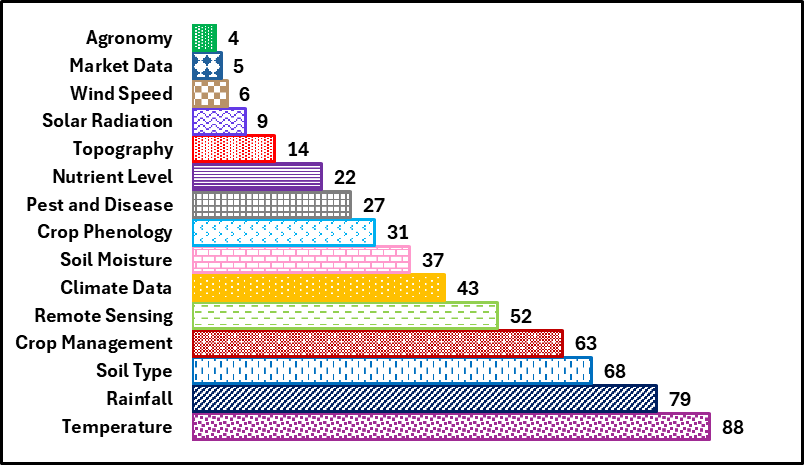
\includegraphics[width=0.8\linewidth]{Frequency.png}
\caption{A Bar Chart Illustrating the Frequency of Key Features Used across the Selected Precision Agriculture Studies (2021-2024)}

\label{fig}
\end{figure}

Fig. 10 shows the frequency of key features across 100 studies on Precision Agriculture. Temperature leads to its usage as the most used feature. With 88 studies utilizing this in developing models. Another variable that is very frequently used is rainfall, which has appeared in 79 studies. Another vital factor is soil type, which is mentioned in 68 studies. Crop management practices are considered in 63 studies and are important in understanding agricultural productivity. Remote sensing data is very important in large-scale, real-time analysis in 52 studies. 

In comparison, general climate data is found in 43 studies. Soil moisture, which indicates water availability, is seen in 37 studies. Crop phenology is used in 31 studies. Pest and disease incidence, affecting crop health and yield, features in 27 studies. Nutrient levels relating to soil fertility are used in 22 studies. Topography, affecting water drainage and soils, is used in 14 studies. Solar radiation, affecting photosynthesis, is used in 9 studies. Wind speed and direction, agronomic practices, and market and economic data occur in 6, 4, and 5 studies, respectively. Underlining their specific but salient roles in certain contexts. This distribution reflects ranges' diversity, which is essential to making a close-to-accurate Crop Yield Prediction.

\section{Grouping by Application Domains, Environment, Contributions, and Specific Problems}

In this section, we group the studies related to Precision Agriculture according to their application domains and environments in which they have been conducted. We also group the contributions to the field and the general-specific problems they help solve. (Fig. 11) This complete grouping also lets us point out trends and underline key findings of previous studies. And, finally we identify gaps that deserve further study. These factors enlighten us on the latest research ground in Precision Agriculture and what underpins ongoing studies.

\begin{figure}[htbp]
\centering
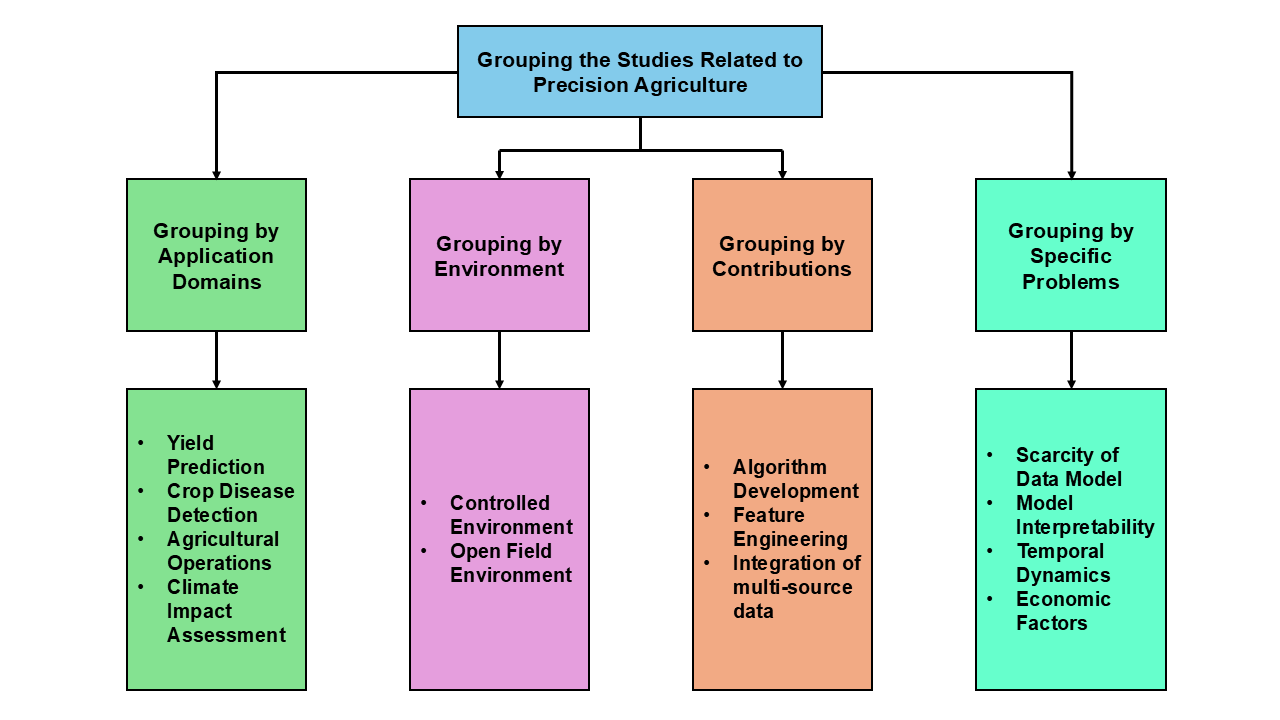
\includegraphics [width= 1\linewidth]{Grouping.png}
\caption{Grouping the Selected Studies Related to Precision Agriculture}
\label{fig}
\end{figure}

\subsection{Grouping by Application Domains}\label{AA}
\textbf{1. Yield Prediction:}
We focus on predicting the yield of several crops, such as wheat, rice, maize, etc. ML and DL algorithms predict crop productivity through weather conditions, soil types, and historical yield data. One important component in this regard is yield prediction. In this case, higher accuracy will mean farmers make better-informed decisions regarding resource allocation and management practices.

\textbf{2. Crop Disease Detection:}
We find the ML and DL algorithms that analyze images and data from different sources in search of early identification and diagnosis of crop diseases \cite{b71}. The eventual outcomes of these algorithms would allow timely intervention and treatment to reduce crop loss and retain overall yield significantly.

\textbf{3. Agricultural Operations:}
We search for optimizing agricultural operations by using prediction models. In simple words, Precision Agriculture implies the observing and regulating of variations in crops, even within a single field, with the aid of technology. This will ultimately lead to higher crop yields and lower costs \cite{b72}.

\textbf{4. Climate Impact Assessment:}
ML and DL algorithms-based research evaluate the impact of climate change on agricultural yields. More importantly, it examines the factors of changing climate variables, especially temperature, rainfall, and CO2 emissions, on Precision Agriculture \cite{b73}. Full awareness of its effects must be created to build adaptive solutions to reduce its impacts on agriculture.

\subsection{Grouping by Environment}

\textbf{1. Controlled Environments:}
Variables such as temperature, humidity, and soil types can be modified in these greenhouse or controlled field experiments to understand variability in crop yields. Controlled environments offer a very homogeneous setting for experiments. They reduce variability due to outer influences on the experiment and increase its reliability.

\textbf{2. Open Field Environments:}
In several studies, we study data from open agricultural fields to capture the complexity and variability of actual farming conditions. The data is gathered from huge farms spanning several different soil types, weather patterns, and management practices. Open field studies are very important for checking the ML and DL algorithm's prediction efficiency in a practical environment with no control over them.

\subsection{Grouping by Contributions}

\textbf{1. Algorithm Development:}
We either find new algorithms or modify the existing ones in the studies. We concentrate on advancing state-of-the-art ML and DL algorithms through innovative approaches or improvements to current models for accuracy, efficiency, and interpretability in precision agriculture.

\textbf{2. Feature Engineering:}
We identify and engineer new features for prediction models. Thus, we prove the importance of effective feature engineering in improving algorithm performance. Feature engineering selects and transforms only relevant data attributes important in Precision Agriculture to enhance accuracy.

\textbf{3. Integration of Multi-source Data:}
Bringing together data sources such as remote sensing and climate data to build full models of the factors that may influence crop yields \cite{b74}. We call for integrating very diverse data to provide a comprehensive view of the agricultural environment and improve prediction.

\subsection{Grouping by Specific Problems}

\textbf{1. Scarcity of Data:} 
We are trying to cope with the limited availability of data and explain how prediction accuracy can be achieved from a small or incomplete dataset. Data augmentation involves creating additional data samples by modifying existing ones. While transfer learning leverages knowledge gained from one task to improve performance on another, often related, task. These regular techniques for coping with scarce data enhance model performance. They are useful for producing synthetic data, which can further expand the dataset and improve the robustness of predictive models.

\textbf{2. Model Interpretability:}
We have seen some attempts to provide complex models with better interpretability by developing algorithms from XAI, which aims to clarify the 'black-box' nature of modern ML and DL algorithms. The term 'black box' refers to models whose internal workings are not easily understood, making it difficult to explain how they arrive at their decisions. Therefore, enhancing interpretability means, first, providing visibility to different stakeholders. It enables them to understand how the model arrived at its decisions, increases confidence in the model, and, most importantly, facilitates practical implementations \cite{b75}.

\textbf{3. Temporal Dynamics:}
This means that temporal changes and seasonality in Precision Agriculture are the main issues these studies address. We have integrated time-series data and temporal modelling methods to capture the dynamics of the agricultural environment \cite{b76}. It may involve algorithms such as RNN and LSTM to be taken for the sake of the trend and seasonality dimension.

\textbf{4. Economic Factors:}
All these studies incorporate economic variables, such as market prices, input costs, and economic indicators, into Crop Yield Prediction models for a complete prediction framework. These attempts to provide a model that embeds both economic factors. These enhance agricultural practice's economic viability and profitability for better decision-making by farmers and policymakers.

\section{Evaluation Metrics used in the Selected Precision Agriculture Studies}

Performance evaluation of Crop Yield Prediction models in Precision Agriculture is usually done using different evaluation metrics. It reflects the accuracy and reliability of results. In the analysis of 100 studies, we find that these evaluation metrics were applied vastly:

% table
\begin{table*}[htbp]
\centering
\caption{Evaluation metrics used in the selected precision agriculture studies}
\begin{adjustbox}{width=\textwidth}
\begin{tabular}{|p{3.5cm}|p{5.5cm}|p{5cm}|}
\hline
\textbf{Evaluation Metrics} & \textbf{Formula} & \textbf{Explanation} \\
\hline
RMSE & 
\[
\text{RMSE} = \sqrt{\frac{1}{n}\sum_{j=1}^{n}( y_j - \hat{y}_j )^2}
\]
& 
$ y_j $ - Actual value,  
$ \hat{y}_j $ - Forecast value,  
$ n $ - Number of observations \\
\hline
MSE & 
\[
\text{MSE} = \frac{1}{n}\sum_{j=1}^{n}( y_j - \hat{y}_j )^2
\]
& 
$ y_j $ - Actual value,  
$ \hat{y}_j $ - Forecast value,  
$ n $ - Number of observations \\
\hline
MAE & 
\[
\text{MAE} = \frac{1}{n}\sum_{j=1}^{n} \left| y_j - \hat{y}_j \right|
\]
& 
$ y_j $ - Actual value,  
$ \hat{y}_j $ - Forecast value,  
$ n $ - Number of observations \\
\hline
MAPE & 
\[
\text{MAPE} = \frac{1}{n}\sum_{j=1}^{n} \left| \frac{y_j - \hat{y}_j}{y_j} \right|
\]
& 
$ y_j $ - Actual value,  
$ \hat{y}_j $ - Forecast value,  
$ n $ - Number of observations \\
\hline
R\(^2\) & 
\[
R^2 = 1 - \frac{\text{RSS}}{\text{TSS}}
\]
& 
RSS - Sum of squares of residuals,  
TSS - Total sum of squares \\
\hline
\end{tabular}
\end{adjustbox}
\label{table:performance_metrics}
\end{table*}

\begin{table*}[htbp]
\centering
\caption{Summary of Evaluation Metrics Used in Some Recently Selected Precision Agriculture Studies}
\begin{adjustbox}{max width=\textwidth}
\begin{tabularx}{\textwidth}{|p{4cm}|X|X|X|X|X|}
\hline
\textbf{Authors} & \textbf{RMSE} & \textbf{MAE} & \textbf{R²} & \textbf{MSE} & \textbf{MAPE} \\
\hline
Rachid Ed-Daoudi et al. (2023) & & & \ding{51} & \ding{51} & \\
\hline
Y. Wang, W. Shi, T. Wen (2023) & & & \ding{51} & & \\
\hline
SANJANA M (2023) & & & \ding{51} & & \\
\hline
Ahmadfaraz Ishaq et al. (2023) & & & \ding{51} & & \\
\hline
Vijayatai Hukare et al. (2023) & \ding{51} & & & \ding{51} & \\
\hline
Jayshree Hajgude, Tanuja Sarode (2023) & \ding{51} & \ding{51} & & \ding{51} & \\
\hline
Qi Zhang et al. (2023) & & & \ding{51} & &  \\
\hline
Dr Kavita Jhajharia, Pratistha Mathur (2024) & & \ding{51} & \ding{51} & \ding{51} & \\
\hline
Subramanian Shanmuga Priya (2023) & \ding{51} & & & & \\
\hline
Yuchi Ma (2023) & & & \ding{51} & & \\
\hline
Venkata Rama Rao Kolipaka (2024) & & \ding{51} & & &\\
\hline
Rajneesh Kumar (2023) & \ding{51} & \ding{51} & \ding{51} & \ding{51} & \\
\hline
Toshihiro Sakamoto (2023) & & & & & \ding{51} \\
\hline
Swanth Boppudi, Sheela J (2024) & & \ding{51} & & \ding{51} & \ding{51} \\
\hline
Parul Setiya, Ajeet Singh Nain, Anurag Satpathi, Mausam IMD (2024) & \ding{51} & \ding{51} & \ding{51} & & \\
\hline
Gowtham Rajendiran, Jebakumar Rethnaraj (2023) & & \ding{51} & \ding{51} & & \\
\hline
Marco Antonio Zanella, Rodrigo Nogueira Martins (2023) & \ding{51} & & \ding{51} & \ding{51} & \\
\hline
Saiara Samira Sajid, Mohsen Shahhosseini, Isaiah Huber (2022) & \ding{51} & & \ding{51} & \ding{51} & \\
\hline
\end{tabularx}
\end{adjustbox}
\end{table*}

\begin{itemize}
\item RMSE
\item MAE
\item R²
\item MSE
\item MAPE
\item CD
\end{itemize}

Now, let us describe each evaluation metric used in the selected Precision Agriculture studies. We also summarize them in TABLE VII \& VIII.

\subsection{RMSE}\label{AA}
RMSE is the square root of the mean of the square of the differences between a model's predictions and the point times series observed. For instance, this RMSE will measure how much, on average, the model predictions are off from the actual values observed. Lower RMSE values indicate better model performance, representing smaller deviations between predicted and observed values. This makes RMSE an important evaluation metric for evaluating the accuracy of Crop Yield Prediction models \cite{b77}. 

Also, it is sensitive to large errors. This turns it into a good metric for developing models so that essential prediction intervals will not go unnoticed. For instance, if large errors accompany Crop Yield Predictions from a model. Then, the RMSE will be high, indicating that model improvement is required.

\subsection{MAE}\label{AA}
MAE calculates or computes the average absolute differences between the predicted and the real values. MAE provides a clear interpretation of prediction accuracy. This makes it a useful metric in scenarios where a uniform margin of error across predictions is preferred, particularly in Crop Yield Prediction.

Furthermore, MAE is less sensitive to outliers than RMSE. Hence, it is suitable when these models have customarily constant type errors \cite{b78}. For example, MAE is used in many studies where constant prediction error is acceptable. Such as estimating the average crop yields of a growing season.

\subsection{R²}\label{AA}
R² is the proportion of variance within the observed data that the model can explain. R² values range from 0 to 1. High values are indicative of good model performance \cite{b79}. R² is widely used in regression analysis. Because it provides a clear indication of how much of the outcome variability can be attributed to the model's input variables.

R² mainly measures the goodness of fit. This means that it measures how well a model explains the variability in data. In Crop Yield Prediction, a high R² value indicates that the model has captured most factors affecting crop yields. 

\subsection{MSE}\label{AA}
MSE is just an average of squared differences between predicted and observed, like RMSE, but without taking the square root. It ensures the same thing as RMSE does but helps when comparing different models applied to the same dataset \cite{b80}. MSE is especially useful when comparing models. It emphasizes significant differences and helps to identify and improve models that may produce larger errors.

It picks out models that are biased to focus on minimizing prediction errors. Thus, it is handy for model selection. MSE penalizes larger errors more severely than smaller ones. It can be particularly effective in highlighting models that consistently produce outliers. This assists in refining model accuracy.

\subsection{MAPE}\label{AA}
MAPE measures the average absolute percentage difference between predicted and observed values. It rescales the errors as a percentage of the observed values. MAPE's ability to normalize errors makes it particularly valuable for comparing prediction performance across diverse datasets. It ensures consistency in accuracy assessment regardless of scale or units.

Because MAPE rescales the errors as a percentage of the actual values, it has advantages in comparing prediction accuracy across different units and target variables. For instance, in crop yield predictions among countries, MAPE allows for a standard assessment of prediction errors across very different kinds of agricultural practice \cite{b81}.

\subsection{CD}\label{AA}
The CD is the proportion of explained variance by the model. The CD is usually used in studies interchangeably with R². It provides a threshold for model performance. Detailing how well it explains the independently realized variability of crop yields \cite{b82}.

\begin{figure}[htbp]
\centering
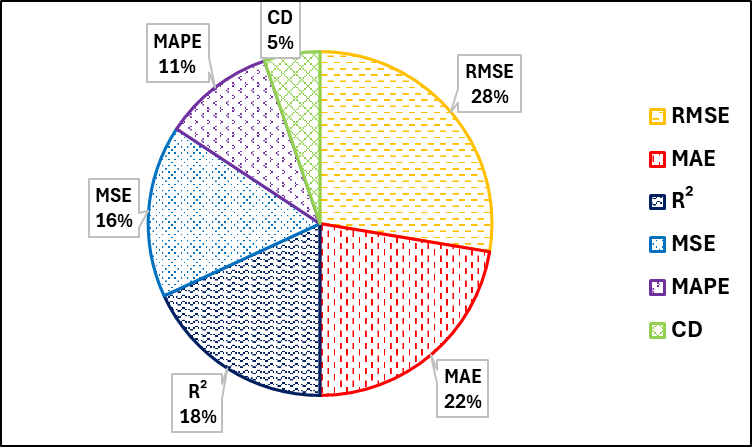
\includegraphics[width=\linewidth]{Number of Studies.png}
\caption{A Pie Chart Illustrating the Number of Studies Using Each Evaluation Metric in the Selected Precision Agriculture Studies (2021-2024)}

\label{fig}
\end{figure}

Fig. 12 gives the idea of 100 studies using various Precision Agriculture research evaluation metrics. Therefore, we find that, RMSE is the most dominant metric used by 58 studies. This shows that it is very important to quantify the average magnitude of prediction errors. In the meantime, 47 studies have used MAE. This is because it gives an easy and direct representation of the average error magnitude. 38 studies have adopted R². Probably because it provides information about the proportion of variance accounted for by the model.

A popular metric is the MSE, featured in 34 studies. At the same time, the MAPE comes in at 22 studies. Making that percentage-based error measure useful for interpretability. The CD is used in 11 studies, which helps to understand how model performance explains data variability.

\section{Challenges and Future Research Directions}
While significant progress has been reported using ML and DL algorithms in Precision Agriculture, many challenges remain. Addressing and summarizing these challenges (Fig. 13 \& TABLE IX) will be essential to further expanding this field and improving the precision and reliability of the models. Future research directions to overcome these challenges are also provided to guide advancements in the Precision Agriculture domain.

\begin{figure}[htbp]
\centering
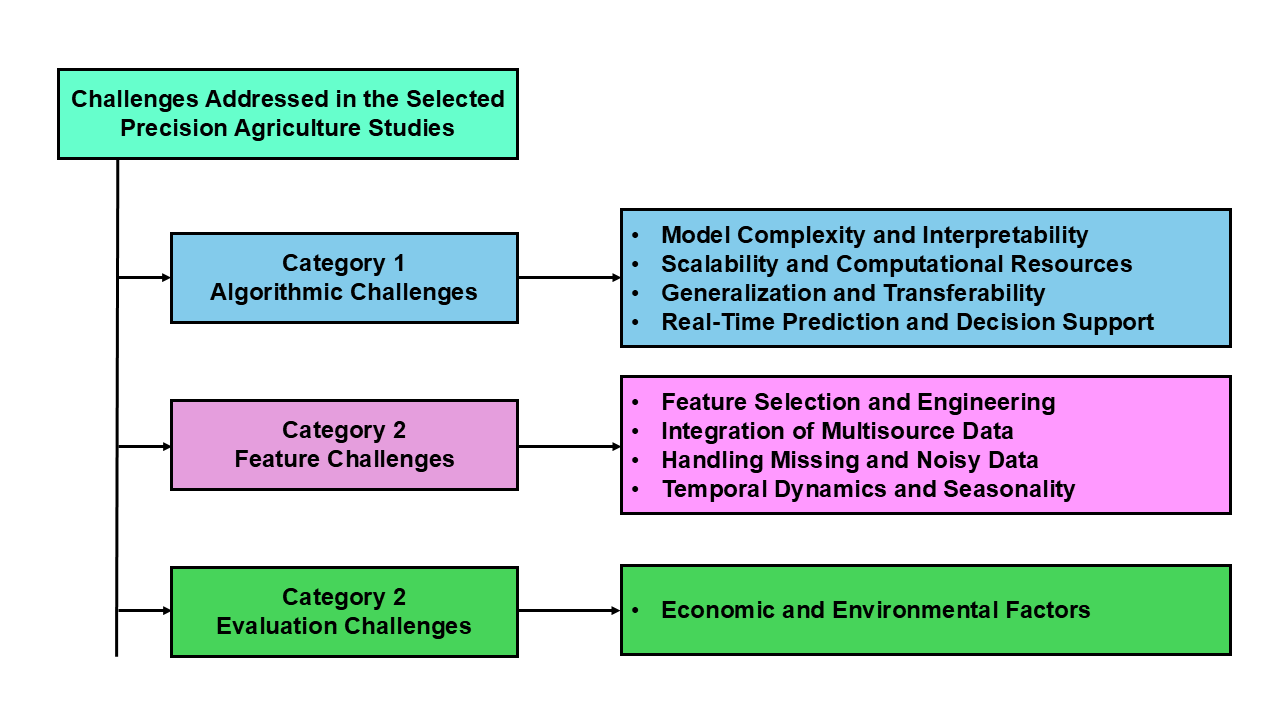
\includegraphics[width= 1\linewidth]{Challenges.png}
\caption{The main challenges in Precision Agriculture, grouped into Algorithmic Challenges, Feature Challenges, and Evaluation Challenges}

\label{fig}
\end{figure}

\begin{table*}[htbp]
\centering
\caption{Challenges Addressed in the Selected Precision Agriculture Studies (2023-2024)}
\begin{adjustbox}{max width=\textwidth}
\begin{tabularx}{\textwidth}{|p{3cm}|X|X|X|X|X|X|X|X|X|}
\hline
\multirow{2}{*}{\textbf{Authors}} & \multicolumn{4}{c|}{\textbf{Algorithmic Challenges}} & \multicolumn{4}{c|}{\textbf{Feature Challenges}} & \multicolumn{1}{c|}{\textbf{Evaluation Challenges}} \\
\cline{2-10} 
& \textbf{Data} & \textbf{Model Int.} & \textbf{Feat. Eng.} & \textbf{Scal.} & \textbf{Gen.} & \textbf{Multi Data} & \textbf{Noisy Data} & \textbf{Season.} & \textbf{Econ.} \\
\hline
Rachid et al. (2023) & \ding{51} &  &  & \ding{51} & \ding{51} & \ding{51} &  &  & \ding{51} \\
\hline
Ying et al. (2023) & \ding{51} & \ding{51} &  &  & \ding{51} &  &  &  & \ding{51} \\
\hline
Marapelli et al. (2023) & \ding{51} &  & \ding{51} & \ding{51} & \ding{51} & \ding{51} &  & \ding{51} &  \\ 
\hline
Sanjana et al. (2023) &  &  &  & \ding{51} & \ding{51} & \ding{51} &  & \ding{51} & \ding{51} \\
\hline
Arpitha et al. (2023) & \ding{51} &  & \ding{51} &  & \ding{51} &  & \ding{51} & \ding{51} &  \\
\hline
Shinde et al. (2023) & \ding{51} &  &  &  & \ding{51} &  & \ding{51} &  &  \\
\hline
Ahmadfaraz et al. (2023) & \ding{51} & \ding{51} & \ding{51} &  &  & \ding{51} & \ding{51} &  & \ding{51} \\
\hline
Moon et al. (2023) &  & \ding{51} &  & \ding{51} & \ding{51} &  &  &  &  \\
\hline
Komati et al. (2023) & \ding{51} & \ding{51} &  &  & \ding{51} & \ding{51} &  &  & \ding{51} \\
\hline
Mildred et al. (2023) & \ding{51} &  &  & \ding{51} & \ding{51} & \ding{51} &  &  & \ding{51} \\
\hline
Vijayatai et al. (2023) & \ding{51} &  &  &  & \ding{51} &  &  & \ding{51} & \ding{51} \\
\hline
Jayshree et al. (2023) & \ding{51} & \ding{51} & \ding{51} & \ding{51} & \ding{51} &  & \ding{51} & \ding{51} & \ding{51} \\
\hline
S. Archana et al. (2023) &  & \ding{51} & \ding{51} & \ding{51} &  & \ding{51} & \ding{51} & \ding{51} &  \\
\hline
Venkata et al. (2024) & \ding{51} &  & \ding{51} & \ding{51} &  & \ding{51} &  & \ding{51} & \ding{51} \\
\hline
Seyed et al. (2023) &  & \ding{51} & \ding{51} & \ding{51} & \ding{51} & \ding{51} & \ding{51} &  & \ding{51} \\
\hline
Dr. Kavita et al. (2024) & \ding{51} & \ding{51} &  & \ding{51} &  & \ding{51} & \ding{51} & \ding{51} & \ding{51} \\
\hline
Subramanian et al. (2023) & \ding{51} &  & \ding{51} & \ding{51} & \ding{51} & \ding{51} &  & \ding{51} & \ding{51} \\
\hline
Yuchi et al. (2023) &  & \ding{51} & \ding{51} &  & \ding{51} &  & \ding{51} &  & \ding{51} \\
\hline
Shevanthe et al. (2023) & \ding{51} &  & \ding{51} &  & \ding{51} &  & \ding{51} & \ding{51} & \ding{51} \\
\hline
Ning et al. (2023) & \ding{51} &  & \ding{51} & \ding{51} &  & \ding{51} & \ding{51} & \ding{51} & \ding{51} \\
\hline
Benjamin et al. (2023) & \ding{51} & \ding{51} & \ding{51} & \ding{51} & \ding{51} & \ding{51} & \ding{51} &  & \ding{51} \\
\hline
Pritesh et al. (2023) & \ding{51} &  &  &  & \ding{51} & \ding{51} &  &  & \ding{51} \\
\hline
Moumita et al. (2023) &  &  & \ding{51} & \ding{51} &  & \ding{51} & \ding{51} &  & \ding{51} \\
\hline
Audrey et al. (2023) & \ding{51} & \ding{51} & \ding{51} & \ding{51} & \ding{51} & \ding{51} & \ding{51} & \ding{51} & \ding{51} \\
\hline
Chigwada et al. (2023) & \ding{51} &  & \ding{51} &  & \ding{51} & \ding{51} & \ding{51} &  &  \\ 
\hline
Kumar et al. (2024) & \ding{51} &  & \ding{51} & \ding{51} & \ding{51} & \ding{51} &  &  & \ding{51} \\ 
\hline
Kalpana et al. (2023) & \ding{51} &  & \ding{51} &  &  & \ding{51} & \ding{51} & \ding{51} &  \\ 
\hline
Deeba et al. (2023) & \ding{51} & \ding{51} & \ding{51} & \ding{51} & \ding{51} &  & \ding{51} &  &  \\ 
\hline
Kallenberg et al. (2023) &  &  & \ding{51} &  & \ding{51} & \ding{51} & \ding{51} &  &  \\ 
\hline
Mahesh et al. (2023) & \ding{51} &  & \ding{51} &  & \ding{51} &  & \ding{51} &  &  \\ 
\hline
Sakamoto et al. (2024) &  & \ding{51} &  & \ding{51} &  & \ding{51} &  & \ding{51} & \ding{51} \\ 
\hline
\end{tabularx}
\end{adjustbox}
\end{table*}

\subsection{Availability and Quality of Data}\label{AA}
Lack of access to high-quality, comprehensive datasets is a major challenge in Precision Agriculture. Data may be incomplete, outdated, or inconsistent, which can reduce model reliability and introduce biases \cite{b83}.

Practical steps to address this include establishing standardized data collection protocols, creating interoperable formats for satellite, soil, and climate data, and promoting collaborative platforms for data sharing. For instance, initiatives like FAO's Agricultural Market Information System enhance transparency and data reliability, supporting more accurate and robust model predictions in real-world applications.

\subsection{Model Complexity and Interpretability}\label{AA}
Advanced ML and DL algorithms, such as DNNs and ensemble methods, are often highly complex and difficult to interpret. While these models can capture intricate patterns in data, their "black-box" nature limits adoption because farmers, agronomists, or policymakers may be reluctant to rely on predictions without understanding the reasoning behind them \cite{b84}.

Future research must center on state-of-the-art XAI techniques to incorporate domain knowledge toward better model transparency. Practical approaches such as rule-based explanations, feature importance ranking, and visual explanations using tools like IBM's AI Explainability 360 toolkit can bridge this gap. This enhances the model’s decision-making process, builds stakeholder trust, and enables more informed, actionable decisions based on model outputs.

\subsection{Feature Selection and Engineering}\label{AA}
Identifying and selecting relevant features is critical yet challenging. Poor feature engineering or sub-optimal selection can mislead decisions, such as irrigation or fertilization planning, and degrade model performance \cite{b85}.

Future research should prioritize automated and robust feature selection techniques that capture spatial and temporal variability in agricultural systems. Features derived from remote sensing, such as vegetation indices, can provide meaningful insights into plant health and stress levels, ensuring decisions are both accurate and actionable.

\subsection{Scalability and Computational Resources}\label{AA}
High computational resources in terms of powerful hardware and extensive computational time are required for training complex models in ML and DL. Inadequate access to these can consequently limit advanced models' full development and field deployment. Especially among researchers and institutions with limited budgets \cite{b86}. 

A very promising future direction will be the use of cloud-based resources coupled with the development of more efficient algorithms that bring down these costs. Google Cloud's scalable AI and ML infrastructure for agriculture provides a perspective on how cloud resources can make that happen. Cloud-based solutions enable the processing of large-scale agricultural data more efficiently. It also reduces the computational burden and allows for real-time insights to improve decision-making and resource allocation.

\subsection{Generalization and Transferability}\label{AA}
Models trained on specific datasets often fail to generalize to other regions, crops, or growing conditions, limiting their broader adoption. Poor generalization can result in inconsistent performance, restricting scalability and practical utility \cite{b87}.

To address this, domain adaptation, multi-region datasets, and fine-tuning strategies can enhance model transferability. For example, a model trained on wheat yields in North America can be adapted to predict rice yields in Asia with minimal retraining. This approach reduces resources needed for deployment in new contexts and enables consistent, reliable performance across diverse agricultural environments.

\subsection{Integration of Multisource Data}\label{AA}
Due to the individual characteristics of satellite imagery, climate data, and other soil-sensing data, heterogeneity in format, resolution, and collection frequency may complicate integration \cite{b88}. Better integration of multisource data is one of the leading factors toward greater model accuracy and robustness. 

One relevant future direction for such development concerns the setting up seamless, harmonizing frameworks in data integration. A concrete example will be satellite images, soil sensors, and climate data properly integrated for accurate Multivariate Analysis (MVA). This integration enables a more holistic understanding of the factors affecting crop yields. This will lead to more accurate predictions and better-informed agricultural decisions. Ultimately enhancing productivity and sustainability.

\subsection{Handling Missing and Noisy Data}\label{AA}
In agricultural datasets, missing and noisy data most of the time exist. This can degrade the model's performance if not handled robustly \cite{b89}. Developing methods that handle such data robustly is needed to guarantee prediction reliability. 

This constitutes a promising future direction for improving data imputation techniques and applying robust methods to handle noisy data. Advanced imputation techniques like matrix factorization will help effectively overcome the missing data issues \cite{b90}. Accurate imputation ensures that subsequent analyses are based on complete and reliable datasets. Eventually, this will lead to more robust and trustworthy predictive models. 

\subsection{Temporal Dynamics and Seasonality}\label{AA}
Temporal dynamics and seasonality in Precision Agriculture are other complex variables. Seasonal dynamics and temporal changes are major challenges for developing models. We have to account for these phenomena to make accurate predictions \cite{b91}. 

Crop Yield Prediction models must include temporal modeling, such as RNNs or LSTMs, to understand seasonal variation. The LSTM algorithm can model crop growth patterns through different seasons. It provides more accurate predictions by considering these temporal dependencies in agricultural data. It allows the model to capture long-term dependencies and trends important for anticipating how crops will respond to changing conditions over time. Thereby, it enhances the reliability of Precision Agriculture.

\subsection{Economic and Environmental Factors}\label{AA}
Integrating economic and environmental considerations into Crop Yield Prediction models is challenging but essential. These factors help ensure that agricultural practices are profitable while minimizing environmental impact \cite{b92}.

Future directions should include incorporating market prices and environmental impact assessments into predictive models. This enables farmers to make decisions that optimize both economic and environmental outcomes, supporting sustainable agriculture and long-term productivity.

\subsection{Real-Time Prediction and Decision Support}\label{AA}
However, such systems that provide farmers with real-time predictions and decision support have been relatively difficult to develop. Such systems require efficient algorithms supported by robust data pipelines that can produce timely and actionable results. 

Therefore, the real focus must be real-time data processing and integration with farm management systems. Real-time data allows farmers to respond rapidly to changing conditions, reduce the risk of crop failure, and optimize resource use. This leads to more resilient and productive agricultural practices. For example, IoT-based real-time crop monitoring tools can enable timely interventions and adjustments. This is for suitability in case immediate feedback is provided to farmers to improve Crop Yield Prediction in Precision Agriculture.

\section{Discussion}

The systematic review of 100 recent Precision Agriculture studies using ML and DL algorithms highlights several important trends, challenges, and opportunities for future research. Our findings show that while the adoption of advanced models such as DNNs, CNNs, LSTMs, and ensemble methods has increased significantly from 2021 to 2024, their performance remains highly dependent on data quality, feature selection, and contextual factors such as region and crop type.

\subsection{Algorithm Performance and Contextual Relevance}

Among ML algorithms, ensemble methods such as Random Forests and Gradient Boosting Machines consistently provide robust performance in scenarios with heterogeneous or incomplete datasets. Traditional methods like Linear Regression and Decision Trees perform reasonably in controlled environments but are often sensitive to noise and outliers. In DL, CNNs and LSTMs demonstrate superior predictive accuracy for remote sensing and time-series datasets, respectively. However, the black-box nature of these models reduces interpretability, limiting stakeholder trust for operational decision-making. Our findings suggest that model selection should not be solely based on accuracy but also consider explainability, data requirements, and operational context.

\subsection{Impact of Data Quality and Scarcity}

Data heterogeneity, scarcity, and quality are critical factors influencing model outcomes. Studies with high-resolution multisource datasets—including IoT, weather, soil, and satellite imagery—show substantially higher prediction accuracy. Conversely, models trained on sparse or incomplete datasets often exhibit poor generalization when applied to new regions or crops. These observations reinforce the need for standardized data collection protocols, collaborative platforms, and open-access repositories to improve model robustness and scalability across diverse agricultural contexts.

\subsection{Regional and Crop-Specific Insights}

Geographic analysis indicates that models developed in Asia and North America dominate the literature, with specific focus on staple crops like rice, wheat, maize, and potatoes. Models trained on one region or crop frequently underperform when applied to other contexts without fine-tuning, highlighting the importance of transfer learning and domain adaptation. For example, models trained on North American wheat data achieve lower accuracy on Asian rice datasets unless adapted through transfer learning strategies. These patterns suggest that future research should prioritize cross-region and cross-crop validation to enhance model generalizability.

\subsection{Practical Implications for Precision Agriculture}

The integration of economic and environmental factors into predictive models is still limited but highly valuable for sustainable decision-making. Models incorporating market prices, resource allocation, and environmental impact indices enable farmers and policymakers to optimize profitability while minimizing ecological consequences. Moreover, explainable AI techniques, such as feature importance analysis and visual model interpretation, are essential for bridging the gap between complex models and actionable insights.

\subsection{Future Directions}

Based on our review, several research directions emerge:

\begin{enumerate}
    \item Development of hybrid ML/DL models that balance predictive accuracy and interpretability.
    \item Expansion of standardized, high-quality, multi-source datasets for global applicability.
    \item Incorporation of domain knowledge and economic/environmental variables into predictive frameworks.
    \item Rigorous cross-region and cross-crop validation to enhance model transferability.
    \item Application of explainable AI to support stakeholder trust and informed decision-making.
\end{enumerate}

Overall, while ML and DL algorithms offer transformative potential for Precision Agriculture, their practical deployment requires careful attention to data quality, interpretability, and contextual relevance. Our review emphasizes that the field is progressing from model-centric development toward holistic, actionable solutions that integrate technology, environmental considerations, and economic decision-making.

\section*{Conclusion}
Our study systematically analyzes the applications of ML and DL algorithms in Precision Agriculture. Through an exhaustive review of 100 studies, we identified the most popular algorithms, key features for model building, and essential evaluation metrics. This comprehensive and state-of-the-art synthesis highlights the strengths and limitations of various algorithms, providing valuable insights for researchers and practitioners in the agricultural and data science communities.

To the best of our knowledge, no other study offers such an extensive examination, making our research a foundational resource in the field. Future research should focus on developing more accurate, robust, and interpretable Precision Agriculture models. Leveraging the latest ML and DL innovations can promote sustainable and productive agricultural practices, enhancing food security and supporting global agricultural development. Our work lays the groundwork for these advancements, fostering collaboration and driving the next generation of predictive models to address the present challenges of food production.

\section*{Clinical Trial Number}
Not applicable.

\section*{Ethics, Consent to Participate, and Consent to Publish Declarations}
Not applicable. 

\section*{Funding Declaration}
Not applicable. 

\section*{Author Contributions}
1. Md. Ashav Noman Mahin: Methodology, Literature Review, Data Collection, Formal Analysis, Visualization, Writing – Original Draft.\\
2. Md. Nasim Adnan: Conceptualization, Review \& Editing, Supervision. \\
3. Rahamatullah Khondoker: Conceptualization, Review \& Editing, Supervision. \\

\section*{Corresponding Author}
Md. Ashav Noman Mahin

\section*{Conflict of Interest}
The authors declare that there are no conflicts of interest regarding the publication of this paper. The research was conducted in the absence of any commercial or financial relationships that could be construed as a potential conflict. All authors have contributed to this work independently and without any external influence that could compromise the integrity or objectivity of this study. The affiliations of the authors are academic and do not reflect any direct industrial partnerships or vested interests in the outcomes presented.

\begin{thebibliography}{00}
\bibitem{b1} Cartwright, M. (2016, May 30). Agriculture in the Fertile Crescent and Mesopotamia. World History Encyclopedia. Retrieved from https://www.worldhistory.org/article/9/agriculture-in-the-fertile-crescent--mesopotamia/
\bibitem{b2} Wang, Ying Shi, Wenjuan Wen, Tianyang. (2023). Prediction of winter wheat yield and dry matter in North China Plain using machine learning algorithms for optimal water and nitrogen application. Agricultural Water Management. 277. 108140. 10.1016/j.agwat.2023.108140. 
\bibitem{b3} Halder, Moon Datta, Ayon Siam, Md Kamrul Mahmud, Shakik Masud, Md Rana, Masud. (2023). A Systematic Review on Crop Yield Prediction Using Machine Learning. ICISN 2023. 668–678. 10.1007/978-981-99-4725-6-77. 
\bibitem{b4} Patel, Pragneshkumar Chaudhary, Sanjay Parmar, Hasit. (2023). Analyze the Impact of Weather Parameters for Crop Yield Prediction Using Deep Learning. 10.1007/978-3-031-24094-2-17.
\bibitem{b5} Science Direct. (2024). Retrieved August 11, 2024, from https://www.sciencedirect.com.
\bibitem{b6} Scopus. (2024). Retrieved August 11, 2024, from https://www.scopus.com.
\bibitem{b7} Web of Science. (2024). Retrieved August 11, 2024, from https://www.webofscience.com.
\bibitem{b8} Springer Link. (2024). Retrieved August 11, 2024, from https://link.springer.com.
\bibitem{b9} Wiley Online Library. (2024). Retrieved August 11, 2024, from https://onlinelibrary.wiley.com.
\bibitem{b10} Google Scholar. (2024). Retrieved August 11, 2024, from https://scholar.google.com.
\bibitem{b11} Sadasivam, Sudha. (2021). Crop Yield Prediction using Granular SVM. International Journal of Recent Technology and Engineering. 9. 85-89. 10.35940/ijrte.F5417.039621. 
\bibitem{b12} Chaudhary, K., Kausar, F. (2020). Prediction of crop yield using machine learning. International Journal of Engineering and Applied Sciences Technology, 4(09), 153-156. 
\bibitem{b13} Deepa, A. Kavya, C. Thomas, Jissy. (2024). Early Prediction of Crop Yield Using Machine Learning Techniques. 10.1007/978-981-99-9707 7-26. 
\bibitem{b14} Shahhosseini, M., Hu, G., Archontoulis, S. V. (2020). Forecasting corn yield with machine learning ensembles. Frontiers in Plant Science, 11, 1120. DOI: 10.3389/fpls.2020.01120. 
\bibitem{b15} Osibo, Benjamin Wahab, Magdy Jia, Li Wenzheng, Ye Bediako Kyeremeh, Bright Osei-Appiah, Stephen. (2023). Interpretable Deep Learning Model for Crop Yield Prediction: A Case Study of Wheat Yield Prediction in Egypt.. 10.21203/rs.3.rs-3020861/v1. 
\bibitem{b16} Hastie, T., Tibshirani, R., Friedman, J. (2009). The Elements of Statisti cal Learning: Data Mining, Inference, and Prediction. Springer Science Business Media. 
\bibitem{b17} P, Ms. (2022). Crop Yield Prediction of Indian Agriculture using Machine Learning Algorithms. International Journal of Advanced Research in Science, Communication and Technology. 685-687. 10.48175/IJARSCT-7035. 
\bibitem{b18} Shahhosseini, M., Hu, G., Archontoulis, S. V. (2020). Forecasting corn yield with machine learning ensembles. Frontiers in Plant Science, 11, 1120. DOI: 10.3389/fpls.2020.01120. 
\bibitem{b19} Athulya, P. Ismail, Mohammed. (2022). Yield Prediction of Indian Crops Based on Weather Data. 10.1007/978-981-19-2004-2-16. 
\bibitem{b20} Gonzalez-Sanchez, A., Frausto-Solis, J., Ojeda-Bustamante, W. (2014). Predictive ability of machine learning methods for massive crop yield prediction. Spanish Journal of Agricultural Research, 12(2), 313–328. 
\bibitem{b21} T R, Mahesh G, Sindhu. (2023). Prediction of Crop Yield Based on Soil Moisture using Machine Learning Algorithms. International Journal of Information Technology, Research and Applications. 2. 33-41. 10.59461/ijitra.v2i1.30. 
\bibitem{b22} Shastry, K. A., Sanjay, H. A., Sajini, M. C. (2022). Decision Tree Based Crop Yield Prediction Using Agro-climatic Parameters. In Emerging Research in Computing, Information, Communication and Applications (pp. 117-125). Springer. 
\bibitem{b23} Gopi, Subbu Karthikeyan, Mani. (2023). Effectiveness of Crop Recommendation and Yield Prediction using Hybrid Moth Flame Optimization with Machine Learning. Engineering, Technology and Applied Science Research. 13. 11360-11365. 10.48084/etasr.6092. 
\bibitem{b24} Darwish, A., El-Askary, H. (2022). Applied Deep Learning-Based Crop Yield Prediction: A Systematic Analysis of Current Developments and Potential Challenges. Technologies, 10(4), 102. DOI: 10.3390/technolo gies10040102. 
\bibitem{b25} Hu, Tongxi Zhang, Xuesong Bohrer, Gil Liu, Yanlan Zhou, Yuyu Martin, Jay Li, Yang Zhao, Kaiguang. (2023). Crop yield prediction via explainable AI and interpretable machine learning: Dangers of black box models for evaluating climate change impacts on crop yield. Agricultural and Forest Meteorology. 336. 109458. 10.1016/j.agrformet.2023.109458. 
\bibitem{b26} Chawla, V. (2022). A Bayesian Network approach to County-Level Corn Yield Prediction using historical data and expert knowledge. arXiv preprint arXiv:1608.05127. 
\bibitem{b27} Patil, Pritesh Athavale, Pranav Bothara, Manas Tambolkar, Siddhi and More, Aditya. (2023). Crop Selection and Yield Prediction using Ma chine Learning Approach. Current Agriculture Research Journal. 11. 968-980. 10.12944/CARJ.11.3.26. 
\bibitem{b28} Bitchi Reddy, B., Chenni Kumaran, J. (2023). A Comparison of the K Nearest Neighbor Algorithm and Naive Bayes for Predicting Agricultural Crop Yield. Journal of Survey in Fisheries Sciences, 10(1S). DOI: 10.17762/sfs.v10i1S.421.
\bibitem{b29} Bhagat, D., Shah, S., Gupta, R.K. (2024). Crop Yield Prediction Using Machine Learning Approaches. Communications in Computer and Information Science, vol 2128. Springer. DOI: 10.1007/978-3-031-62217 5-6. 
\bibitem{b30} Mohamed A. Mattar and Ahmed A. El-Shafei (2021). Groundwater Level Prediction Using a Multiple Objective Genetic Algorithm-Grey Relational Analysis Based Weighted Ensemble of ANFIS Models. Water, 13(21), 3130. DOI: 10.3390/w13213130. 
\bibitem{b31} Reddy, Kandi Reddy, Evuri. (2023). Crop Yield Prediction Based on Weather and Soil Parameters Using Regression Tree Model. 10.1007/978-981-99-2710-4-1. 
\bibitem{b32} Khazaei, J., Naghavi, M. R., Jahansouz, M. R., Salimi-Khorshidi, G. (2008). Yield estimation and clustering of chickpea genotypes using soft computing techniques. Agronomy Journal, 100(4), 1077–1087. DOI: 10.2134/agronj2007.0318. 
\bibitem{b33} Setiya, Parul Nain, Ajeet Satpathi, Anurag IMD, Mausam. (2024). Comparative analysis of SMLR, ANN, Elastic net and LASSO based models for rice crop yield prediction in Uttarakhand. MAUSAM. 75. 191-196. 10.54302/mausam.v75i1.3576. 
\bibitem{b34} Khaki, S., Wang, L. (2019). Crop yield prediction using deep neural networks. Frontiers in Plant Science, 10, 621. DOI: 10.3389/fpls.2019.00621. 
\bibitem{b35} Gopal, P.S.M., Bhargavi, R. (2019). A novel approach for efficient crop yield prediction. Computers and Electronics in Agriculture, 165, 104968. DOI: 10.1016/j.compag.2019.104968. 
\bibitem{b36} Gopi, P. Karthikeyan, M.. (2023). Red fox optimization with ensemble recurrent neural network for crop recommendation and yield prediction model. Multimedia Tools and Applications. 83. 1-21. 10.1007/s11042 023-16113-2. 
\bibitem{b37} Muruganantham, P., Wibowo, S., Grandhi, S., Samrat, N.H., Islam, N. (2023). Deep Learning-Based Crop Yield Prediction Using RNNs. MDPI Sensors. DOI: 10.3390/s22062307. 
\bibitem{b38} Kallenberg, Michiel Maestrini, Bernardo van Bree, Ron Ravensbergen, A. P. P. Pylianidis, Christos van Evert, Frits Athanasiadis, Ioannis. (2023). Integrating processed-based models and machine learning for crop yield prediction.
\bibitem{b39} Shanmugam, Iniyan Rethnaraj, Jebakumar Mani, Gayathri. (2023). Selection of crop varieties and yield prediction based on phenotype applying deep learning. International Journal of Electrical and Computer Engineering (IJECE). 13. 6806. 10.11591/ijece.v13i6.pp6806-6816. 
\bibitem{b40} Jiang, Z., Liu, C., Ganapathysubramanian, B., Sarkar, S. (2020). Predicting County-Scale Maize Yields with LSTM Networks Using Weather and Soil Data. Scientific Reports, 10(1), 1-12. DOI: 10.1038/s41598 020-65647-4. 
\bibitem{b41} Kalaiarasi, E. (2021). Crop yield prediction using multi-parametric deep neural networks. Indian Journal of Science and Technology. 14. 131-140. 10.17485/IJST/v14i2.2115. 
\bibitem{b42} Sjølander, B. L. O., et al. (2021). Farm-Scale Crop Yield Prediction from Multi-Temporal Data Using Deep Hybrid Neural Networks. Agronomy, 11(12), 2576. DOI: 10.3390/agronomy11122576. 
\bibitem{b43} USDA Foreign Agricultural Service. India: Grain and Feed Annual. (2023). Available at: USDA FAS. 
\bibitem{b44} Munasinghe, Hashini Dasunika, Tyni Subhodani, Lakshika Janotheepan, M Ekanayake, Jayalath Perera, Nilusha. (2023). Development of Crop Yield Prediction Model Using Machine Learning Algorithms: A Review.  
\bibitem{b45} Lobell, D., Cahill, K., Field, C. B. (2007). Historical effects of temperature and precipitation on California crop yields. Stanford FSI. 
\bibitem{b46} Marapelli, Bhaskar Anamalamudi, Lokeshwari Potluri, Chandra Carie, Anil Anamalamudi, Satish. (2023). Enhancing Agricultural Decision Making Through Machine Learning-Based Crop Yield Predictions. 10.1007/978-981-99-6755-1-16. 
\bibitem{b47} Barati, M.K., et al. (2022). ”Rainfall Variability and Rice Sustainability: An Evaluation Study of Two Distinct Rice-Growing Ecosystems.” MDPI Land, 11(8), 1242. DOI: 10.3390/land11081242. 
\bibitem{b48} Shanmugam, Iniyan Rethnaraj, Jebakumar Rajendran, Srinivasan Senthilraja, M.. (2023). Prediction on field crops yield based on analysis of deep learning model. Indonesian Journal of Electrical Engineering and Computer Science. 30. 518. 10.11591/ijeecs.v30.i1.pp518-527. 
\bibitem{b49} Bhattacharyya, T., et al. ”Agro-ecological Regions for Better Crop Planning and Ecosystem Services.” SpringerLink. 
\bibitem{b50} Yang, Meijian Wang, Guiling Wu, Shu Block, Paul Lazin, Rehenuma Alexander, Sarah Lala, Jonathan Haider, Muhammad Rezaul Dokou, Zoi Atsbeha, Ezana Koukoula, Marika Shen, Xinyi Pe˜ na, Malaquias Nikolopoulos, Efthymios Bagtzoglou, Amvrossios Anagnostou, Em manouil. (2023). Seasonal prediction of crop yields in Ethiopia using an analog approach. Agricultural and Forest Meteorology. 331. 109347. 10.1016/j.agrformet.2023.109347.
\bibitem{b51} CSIRO. Wheatcast: Wheat Yield Forecasts for Australia. CSIRO Digiscape Future Science Platform. 
\bibitem{b52} Salokhe, Mayur. (2023). Machine Learning: Applications in Agriculture (Crop Yield Prediction, Diease and Pest Detection). International Journal of Advanced Research in Science, Communication and Technology. 592 597. 10.48175/IJARSCT-12088. 
\bibitem{b53} Abendroth, L., Elmore, R. (2024). ”Planting Date Trends.” Iowa State University, Integrated Crop Management. 
\bibitem{b54} Bregaglio, Simone Ginaldi, Fabrizio Raparelli, Elisabetta Fila, Gianni Bajocco, Sofia. (2023). Improving crop yield prediction accuracy by embedding phenological heterogeneity into model parameter sets. Agri cultural Systems. 209. 103666. 10.1016/j.agsy.2023.103666.
\bibitem{b55} Santana, C. T. C., Sanches, I. D., Caldas, M. M., Adami, M. (2024). A Method for Estimating Soybean Sowing, Beginning Seed, and Harvesting Dates in Brazil Using NDVI-MODIS Data. Remote Sensing, 16(14), 2520. DOI: 10.3390/rs16142520.
\bibitem{b56}  M. Talaat, Fatma. (2023). Crop yield prediction algorithm (CYPA) in precision agriculture based on IoT techniques and climate changes. Neural Computing and Applications. 35. 10.1007/s00521-023-08619-5.
\bibitem{b57} Ag Alert. Sensors guide growers on water decisions. Ag Alert, California Farm Bureau Federation. 
\bibitem{b58} Amankulova, Khilola Farmonov, Nizom Uzbekhon, Mukhtorov Mucsi, Laszlo. (2023). Sunflower crop yield prediction by advanced statistical modeling using satellite-derived vegetation indices and crop phenology. Geocarto International. 38. 1-23. 10.1080/10106049.2023.2197509. 
\bibitem{b59} Wolkovich, E. M., et al. (2022). Exploring Grapevine Phenology and High Temperatures Response Under Controlled Conditions. Frontiers in Plant Science. 
\bibitem{b60} L´opez Segura, Mildred Lasserre, Alberto Fern´ andez Lambert, Gre gorio G´omez, Rub´en V´asquez, Daniel. (2023). XGBoost sequential system for the prediction of Persian lemon crop yield. Crop Science. 10.1002/csc2.21148. 
\bibitem{b61} IntechOpen (2021). Managing a Transboundary Pest: The Fall Army worm on Maize in Africa. 
\bibitem{b62} Venkatesh, Kummari Naik, K. Jairam. (2024). An ensemble transfer learning for nutrient deficiency identification and yield-loss prediction in crop. Multimedia Tools and Applications. 1-27. 10.1007/s11042-024 18592-3.  
\bibitem{b63} Li, X., Hu, X., Song, S. (2024). ”Greenhouse Management for Better Vegetable Quality, Higher Nutrient Use Efficiency, and Healthier Soil.” Horticulturae, 10(1), 49. DOI: 10.3390/horticulturae10010049. 
\bibitem{b64} Zimmerer, K. S. (1996). Changing Fortunes: Biodiversity and Peasant Livelihood in the Peruvian Andes. University of California Press, Berkeley, CA. 
\bibitem{b65} Mariscal, M. J., Orgaz, F., Villalobos, F. J. (2000). Radiation-Use Efficiency and Dry Matter Partitioning of Olive (Olea europaea) Trees. Tree Physiology. 
\bibitem{b66} Top Crop Manager. Wind Erosion Remains a Problem on the Prairies. Top Crop Manager, 2021.  
\bibitem{b67} Shivalingaiah, Santhosh Umesh, Kattekyathanalli. (2023). AN ENSEM BLEAPPROACHFORCOFFEECROPYIELDPREDICTIONBASED ONAGRONOMICFACTORS.ASEANEngineering Journal. 13. 29-38. 10.11113/aej.v13.18846. 
\bibitem{b68} Haelterman, T. (2020). No-till farming improves crop yields, study finds. Spartan Newsroom. 
\bibitem{b69} Kalpana, P Prem, I Mary, S Rani, ArockiaValan. (2023). Crop Yield Prediction Using Machine Learning. REST Journal on Data Analytics and Artificial Intelligence. 2. 16-20. 10.46632/jdaai/2/1/3. 
\bibitem{b70} KIPPRA. Enhancing Market Access Through Digital Technologies Among Smallholder Farmers in Kenya. Kenya Institute for Public Policy Research and Analysis (KIPPRA).
\bibitem{b71} Momenpour, Seyed Bazgeer, Saeed Moghbel, Masoumeh. (2024). A bibliometric analysis of the literature on crop yield prediction: insights from previous findings and prospects for future research. International journal of biometeorology. 68. 10.1007/s00484-024-02628-2.
\bibitem{b72} Shawon, Sarowar Ema, Falguny Mahi, Asura Raihan, Md. Mohsin. (2023). Crop Yield Prediction: Robust Machine Learning Approaches for Precision Agriculture. 1-6. 10.1109/ICCIT60459.2023.10441634. 
\bibitem{b73} Klompenburg, Thomas Kassahun, Ayalew Catal, Cagatay. (2020). Crop yield prediction using machine learning: A systematic literature review. Computers and Electronics in Agriculture. 177. 105709. 10.1016/j.compag.2020.105709.
\bibitem{b74} Ishaq, Rana Zhou, Guanhua Tian, Chen Tan, Yumin Jing, Guifei Jiang, Hongzhi, Obaid-ur-Rehman. (2023). A Systematic Review of Radiative Transfer Models for Crop Yield Prediction and Crop Traits Retrieval. Remote Sensing. 16. 10.3390/rs16010121. 
\bibitem{b75} Chang, Yanbin Latham, Jeremy Licht, Mark Wang, Lizhi. (2023). A data-driven crop model for maize yield prediction. Communications Biology. 6. 10.1038/s42003-023-04833-y. 
\bibitem{b76} Dey, Tanushree Bera, Somnath Paul, Bachchu De, Debashis Mukherjee, Anwesha Buyya, Rajkumar. (2024). Fly: Femtolet-based edge-cloud framework for crop yield prediction using bidirectional long short-term memory. Software: Practice and Experience. 54. 10.1002/spe.3324.
\bibitem{b77} Sajid, Saiara Shahhosseini, Mohsen Huber, Isaiah Hu, Guiping Archontoulis, Sotirios. (2022). County-scale crop yield prediction by integrating crop simulation with machine learning models. Frontiers in Plant Science. 13. 10.3389/fpls.2022.1000224. 
\bibitem{b78} Zhao, Yanxi Xiao, Dengpan Huizi, Bai Tang, Jianzhao Qi, Yongqing Shen, Yanjun. (2023). The Prediction of Wheat Yield in the North China Plain by Coupling Crop Model with Machine Learning Algorithms. Agriculture. 13. 99. 10.3390/agriculture13010099. 
\bibitem{b79} Tian, Zezhong Zhang, Yao Liu, Kaidi Li, Zhenhai Li, Minzan Zhang, Haiyang Wu, Jiangmei Uav,. (2022). Remote Sensing Prediction Method of Winter Wheat Yield Based on the Fused Features of Crop and Soil. 10.3390/rs14195054. 
\bibitem{b80} ansari far, Javad Wang, Lizhi Archontoulis, Sotirios. (2021). An interaction regression model for crop yield prediction. Scientific Reports. 11. 10.1038/s41598-021-97221-7. 
\bibitem{b81} Nyéki, A., Neményi, M. (2022). Crop Yield Prediction in Precision Agriculture. Agronomy, 12(10), 2460. MDPI.
\bibitem{b82} Cen, H., Wan, L. (2023). Crop Yield Estimation and Prediction. Encyclopedia of Smart Agriculture Technologies. Springer, Cham. DOI: 10.1007/978-3-030-89123-7-48-1.
\bibitem{b83} Pandya, Parthsarthi Gontia, Narendra Kumar. (2023). Early crop yield prediction for agricultural drought monitoring using drought indices, remote sensing, and machine learning techniques. Journal of Water and Climate Change. 14. 10.2166/wcc.2023.386. 
\bibitem{b84} Zanella, Marco Martins, Rodrigo Silva, Fábio Carvalho, Luis Alves, Marcelo Fim Rosas, Jorge. (2023). Coffee yield prediction using high-resolution satellite imagery and crop nutritional status in Southeast Brazil. Remote Sensing Applications Society and Environment. 33. 101092. 10.1016/j.rsase.2023.101092. 
\bibitem{b85} Hajgude, Jayshree Sarode, Tanuja. (2023). Comparative Study of Ensemble Models for the Prediction of Crop Yield. 10.1007/978-981-99-3485-0-30. 
\bibitem{b86} Sakamoto, Toshihiro. (2024). Crop Monitoring System Using MODIS Time-Series Data for Within-Season Prediction of Yield and Production of US Corn and Soybeans. Photogrammetric Engineering and Remote Sensing. 90. 99-119. 10.14358/PERS.23-00052R2. 
\bibitem{b87} Zhang, Qi Wang, Kaiyi Han, Hanyun Liu, Zhongqiang Yang, Feng Wang, Shufeng Zhao, Xiangyu Zhao, Chunjiang. (2022). A crop variety yield prediction system based on variety yield data compensation. Computers and Electronics in Agriculture. 203. 107460. 10.1016/j.compag.2022.107460. 
\bibitem{b88} Saludares, Rica Amor Atanda, Sikiru Piche, Lisa Worral, Hannah Dariva, Françoise Mcphee, Kevin Bandillo, Nonoy. (2024). Multi-trait multi-environment genomic prediction of preliminary yield trials in pulse crops. 10.1101/2024.02.18.580909. 
\bibitem{b89} Bagheri, Saghar Cheung, Gene Eadie, Tim. (2023). Graph Sparsification for GCN Towards Optimal Crop Yield Predictions.
\bibitem{b90} Sengupta, S., Tam, L., Wu, P., Dasgupta, S.,  Udell, M. (2017). "A Matrix Factorization Approach to Data Imputation." Stanford University.
\bibitem{b91} T., Padma, Sinha, Dipali. (2023). Crop Yield Prediction Using Improved Random Forest. ITM Web of Conferences. 56. 10.1051/itmconf/20235602007. 
\bibitem{b92} Swain, Debabrata Lakum, Sachin Patel, Samrat Patro, Pramoda Jatin,. (2024). An Efficient Crop Yield Prediction System Using Machine Learning. EAI Endorsed Transactions on Internet of Things. 10. 10.4108/eetiot.5333. 
\bibitem{b93} Rajendiran, Gowtham Rethnaraj, Jebakumar. (2023). Lettuce Crop Yield Prediction Analysis using Random Forest Regression Machine Learning Model in Aeroponics System. 565-572. 10.1109/ICAISS58487.2023.10250535. 
\bibitem{b94} Bibi, Maryum Rehman, Saif Mahmood, Khalid. (2023). An Intelligent Decision Support System for Crop Yield Prediction Using Machine Learning and Deep Learning Algorithms. Proceedings of the Pakistan Academy of Sciences: A. Physical and Computational Sciences. 60. 10.53560/PPASA(60-3)825. 
\bibitem{b95} Zhang, Yuanmin Liao, Yule Li, Yanjun. (2023). A new method of crop yield prediction based on artificial intelligence. Journal of Physics: Conference Series. 2665. 012019. 10.1088/1742-6596/2665/1/012019. 
\bibitem{b96} Kolipaka, Venkata Namburu, Anupama. (2024). Hybrid Classification Model with Tuned Weights for Crop Yield Prediction. Wireless Personal Communications. 133. 1-23. 10.1007/s11277-023-10781-x. 
\bibitem{b97} Taşkıner, Tuğçe Bilgen, Bilge. (2021). Optimization Models for Harvest and Production Planning in Agri-Food Supply Chain: A Systematic Review. Logistics. 5. 52. 10.3390/logistics5030052. 
\bibitem{b98} Chen, Jiang Yu, Tong Cherney, Jerome Zhang, Zhou. (2024). Optimal Integration of Optical and SAR Data for Improving Alfalfa Yield and Quality Traits Prediction: New Insights into Satellite-Based Forage Crop Monitoring. Remote Sensing. 16. 734. 10.3390/rs16050734. 
\bibitem{b99} S, Thirumal, R, Latha. (2023). Teaching and Learning based Optimization with Deep Learning Model for Rice Crop Yield Prediction. International Journal of Electrical and Electronics Engineering. 10. 105-114. 10.14445/23488379/IJEEE-V10I4P110. 
\bibitem{b100} Satish, Prof. (2023). Crop Yield Prediction using GELM (Gaussian Extreme Learning Machine). INTERNATIONAL JOURNAL OF SCIENTIFIC RESEARCH IN ENGINEERING AND MANAGEMENT. 07. 1-10. 10.55041/IJSREM27485. 
\bibitem{b101} Ma, Yuchi Yang, Zhengwei Huang, Qunying Zhang, Zhou. (2023). Improving the Transferability of Deep Learning Models for Crop Yield Prediction: A Partial Domain Adaptation Approach. Remote Sensing. 15. 10.3390/rs15184562. 
\bibitem{b102} Narawade, Vaibhav Chaudhari, Akash Mohammad, Muntazir Dubey, Tanmay Jadhav, Bhumika. (2024). Agricultural Crop Yield Prediction for Indian Farmers Using Machine Learning. 10.1007/978-981-99-8476-3-7. 
\bibitem{b103} Chaiyana, Akkarapon Hanchoowong, Ratchawatch Srihanu, Neti Prasanchum, Haris Kangrang, Anongrit Hormwichian, Rattana Kaewplang, Siwa Koedsin, Werapong Huete, Alfredo. (2024). Leveraging Remotely Sensed and Climatic Data for Improved Crop Yield Prediction in the Chi Basin, Thailand. Sustainability. 16. 2260. 10.3390/su16062260. 
\bibitem{b104} M, SANJANA. (2023). CROP YIELD PREDICTION BASED ON MACHINE LEARNING. INTERNATIONAL JOURNAL OF SCIENTIFIC RESEARCH IN ENGINEERING AND MANAGEMENT. 07. 10.55041/IJSREM24714. 
\bibitem{b105} L. R.Meena (2020). Crop-based integrated farming systems for sustainable production, nutritional security, and environmental safeguard. Science for Agriculture and Allied Sector. 2582-368X.
\bibitem{b106} Kumar, V. Ramesh, K. Rakesh, V.. (2023). Optimizing LSTM and Bi‑LSTM models for crop yield prediction and comparison of their performance with traditional machine learning techniques. Applied Intelligence. 10.1007/s10489-023-05005-5. 
\bibitem{b107} Joshi, Abhasha Pradhan, Biswajeet Gite, Shilpa Chakraborty, Subrata. (2023). Remote-Sensing Data and Deep-Learning Techniques in Crop Mapping and Yield Prediction: A Systematic Review. Remote Sensing. 15. 10.3390/rs15082014. 
\bibitem{b108} Boppudi, Swanth J, Sheela. (2024). Deep ensemble model with hybrid intelligence technique for crop yield prediction. Multimedia Tools and Applications. 1-21. 10.1007/s11042-024-18354-1. 
\bibitem{b109} Wang, Ning Zhong, Ma Huo, Pengcheng Liu, Xi He, Zhao Lu, Kedi. (2023). 3D Convolutional Neural Network with Dimension Reduction and Metric Learning for Crop Yield Prediction Based on Remote Sensing Data. Applied Sciences. 13. 13305. 10.3390/app132413305. 
\bibitem{b110} Al-Shammari, Dhahi Bishop, Thomas Wang, Chen Whelan, Brett Bramley, Robert. (2022). A comparison between machine learning and simple mechanistic-type models for yield prediction in site-specific crop yield predictions.
\bibitem{b111} Liu, Qinqing Dou, Fei Yang, Meijian Amdework, Ezana Wang, Guiling Bi, Jinbo. (2023). Customized Positional Encoding to Combine Static and Time-varying Data in Robust Representation Learning for Crop Yield Prediction. 6094-6102. 10.24963/ijcai.2023/676. 
\bibitem{b112} Yeşilköy, Serhan Demir, Ibrahim. (2023). Crop Yield Prediction based on Reanalysis and Crop Phenology Data in the Agroclimatic Zones. 10.31223/X5BW8H. 
\bibitem{b113} Moswa, Audrey Killeen, Patrick Kiringa, Iluju Yeap, Tet. (2023). Corn Yield Prediction Using Crop Growth and Machine Learning Models. 10.1007/978-981-99-1203-2-28. 
\bibitem{b114} Modepalli, Kavitha. (2021). An Ensemble Algorithm for Crop Yield Prediction. 
\bibitem{b115} Chaudhary, Yashi Pathak, Heman. (2024). CYPBL: Crop Yield Prediction using Bi-Directional LSTM under PySpark interface. Multimedia Tools and Applications. 1-20. 10.1007/s11042-024-18638-6. 
\bibitem{b116} Oshodi, Ismaila. (2023). DEVELOPMENT OF MACHINE LEARNING ALGORITHMS FOR IMPROVING CROP YIELD PREDICTION by ISMAILA OSHODI. 10.13140/RG.2.2.35258.57281. 
\bibitem{b117} Ahmed, Abdulbasit Adewumi, Sunday Yemi-Peters, Victoria. (2023). Seasonal Crop Yield Prediction in Nigeria Using Machine Learning Technique. Journal of Applied Artificial Intelligence. 4. 10.48185/jaai.v4i1.728. 
\bibitem{b118} Kolipaka, Venkata Namburu, Anupama. (2023). An automatic crop yield prediction framework designed with two-stage classifiers: a meta-heuristic approach. Multimedia Tools and Applications. 83. 1-24. 10.1007/s11042-023-16612-2. 
\bibitem{b119} Jhajharia, Dr Mathur, Pratistha. (2024). Machine Learning Based Crop Yield Prediction Model in Rajasthan Region of India. Iraqi Journal of Science. 390-400. 10.24996/ijs.2024.65.1.32.
\bibitem{b120} Muruganantham, Priyanga Wibowo, Santoso Grandhi, Sriman Samrat, Nahidul Islam, Nahina. (2022). A Systematic Literature Review on Crop Yield Prediction with Deep Learning and Remote Sensing. Remote Sensing. 14. 1990. 10.3390/rs14091990. 
\bibitem{b121} Rahman, Sajjadur Rubab, Md. Mashrur Hossain Payal, Mahjabin. (2023). Improving Crop Productivity in Bangladesh Through Advanced Yield Prediction Techniques. 10.13140/RG.2.2.16907.36644. 
\bibitem{b122} Shivnanda, Shinde Nikita, Pawar Tanaji, Dhage. (2023). Yield Predict: A Crop Yield Prediction Framework for Smart Farms. International Journal of Advanced Research in Science, Communication and Technology. 539-541. 10.48175/IJARSCT-14078. 
\bibitem{b123} Rashid, Mamunur Bari, Bifta Yusup, Yusri Kamaruddin, Mohamad Khan, Nuzhat. (2021). A Comprehensive Review of Crop Yield Prediction Using Machine Learning Approaches With Special Emphasis on Palm Oil Yield Prediction. IEEE Access. 9. 10.1109/ACCESS.2021.3075159. 
\bibitem{b124} Ed-Daoudi, Rachid Alaoui, Altaf Ettaki, Badia Zerouaoui, Jamal. (2023). Improving Crop Yield Predictions in Morocco Using Machine Learning Algorithms. Journal of Ecological Engineering. 24. 392–400. 10.12911/22998993/162769. 
\bibitem{b125} Sekar, Shevanthe E, Sathiyamoorthy. (2023). A SYSTEMATIC STUDY ABOUT THE CROP YIELD PREDICTION WITH MACHINE LEARNING TECHNIQUES. Journal of Survey in Fisheries Sciences. 2477-2496. 10.53555/sfs.v10i1.489. 
\bibitem{b126} Hukare, Vijayatai Kumbhar -Patkar, Vidya Shah, Sahil. (2023). Machine Learning Methods for Crop Yield Prediction. 10.1007/978-3-031-43605-5-15. 
\bibitem{b127} Kumar, Rajneesh Mahapatra, Rajendra. (2024). Severity of natural calamities and crop yield prediction using hybrid deep learning model in Uttar Pradesh. World Water Policy. 10. 244-279. 10.1002/wwp2.12163. 
\bibitem{b128} Sivanantham, V. Sangeetha, V. Ali, Abeer Hatamleh, Wesam Chunduru, Anilkumar Hatamleh, Ashraf Sweidan, Dirar. (2022). Quantile correlative deep feedforward multilayer perceptron for crop yield prediction. Computers and Electrical Engineering. 98. 107696. 10.1016/j.compeleceng.2022.107696. 
\bibitem{b129} Shanmuga priya, Subramanian Dathan, R. (2023). Attention based Peephole LSTM model for Soybean crop yield prediction. Journal of Physics: Conference Series. 2571. 012013. 10.1088/1742-6596/2571/1/012013. 
\bibitem{b130} Pande, Shilpa. (2020). Towards a Unified Approach for Crop Yield Prediction. International Journal of Emerging Trends in Engineering Research. 8. 3236-3240. 10.30534/ijeter/2020/58872020. 
\bibitem{b131} Goswami, Moumita Bhattacharjee, Sanghita Changder, Suvamoy. (2023). A Novel Approach for Crop Yield Prediction Model Validation. 10.56155/978-81-955020-2-8-10. 
\bibitem{b132} Chigwada, Thobekile Dzinomwa, Mary Mutunhu Ndlovu, Belinda Sibanda, Khulekani Moyo, Sibonile. (2023). Maize Crop Yield Prediction Model Using Machine Learning. 10.46254/AP04.20230046. 
\bibitem{b133} Krupavath, K. Babu, M. Mani, Adusumilli. (2022). Comparative Evaluation of Neural Networks in Crop Yield Prediction of Paddy and Sugarcane Crop. 10.1002/9781119823469.ch2. 
\bibitem{b134} Sukriti, Pandey, Kamal Danodia, Abhishek Harish, Chandra Karnatak, Harish. (2023). Development of Machine Learning based Models for Multivariate Prediction of Wheat Crop Yield in Uttar Pradesh, India. Journal of Geomatics. 17. 94-101. 10.58825/jog.2023.17.2.70. 
\bibitem{b135} Kumar, Rajneesh Pandey, Sachi. (2022). An accurate prediction of crop yield using hybrid deep capsule auto encoder with softmax regression. Multimedia Tools and Applications. 82. 10.1007/s11042-022-13919-4. 
\bibitem{b136} Rao, Raghavendra. (2022). CROP YIELD PREDICTION USING MACHINE LEARNING ALGORITHMS. International Journal of Innovative Research in Advanced Engineering. 09. 502-505. 10.26562/ijirae.2022.v0906.08.
\bibitem{b137} Kolipaka, Venkata Namburu, Anupama. (2023). Integrating Temporal Fluctuations in Crop Growth with Stacked Bidirectional LSTM and 3D CNN Fusion for Enhanced Crop Yield Prediction. International Journal on Recent and Innovation Trends in Computing and Communication. 11. 376-383. 10.17762/ijritcc.v11i9.8543. 
\bibitem{b138} Varghese, Arpitha Inna, Mamatha. (2023). A Unified System for Crop Yield Prediction, Crop Recommendation, and Crop Disease Detection. 10.1007/978-981-99-4634-1-81. 
\bibitem{b139} Albaaji, Ghassan Sreelakshmi, S Chandra, Vinod. (2023). Crop Yield Prediction for Smart Agriculture with Climatic Parameters Using Random Forest. 10.1007/978-3-031-37940-6-30. 
\bibitem{b140} Aggarwal, Ashwani Jaidka, Preeti. (2022). Segmentation of Crop Images for Crop Yield Prediction. 
\bibitem{b141} Deeba, Devi, O Bhargavi, Peddi Reddy, Manohara, El-Ebiary, Yousef Rengarajan, Manikandan Al Ansari, Dr. Mohammed Saleh. (2023). Optimizing Crop Yield Prediction in Precision Agriculture with Hyperspectral Imaging-Unmixing and Deep Learning. International Journal of Advanced Computer Science and Applications. 14. 10.14569/IJACSA.2023.0141261. 
\bibitem{b142} Ip, Ryan Ho Leung Ang, Li-Minn Seng, Kah Broster, John Pratley, James. (2018). Big data and machine learning for crop protection. Computers and Electronics in Agriculture. 151. 376-383. 10.1016/j.compag.2018.06.008. 
\bibitem{b143}Archana, S. Paramasivan, Senthil. (2023). A Survey on Deep Learning Based Crop Yield Prediction. Nature Environment and Pollution Technology. 22. 579-592. 10.46488/NEPT.2023.v22i02.004. 
\bibitem{b144} Author, Kumar, Pradeep Srimathi, K Gulaiya, Shani Ojha, Rahul. (2024). Precision Agriculture and Smart Farming. 
\bibitem{b145} Mgendi, George. (2024). Unlocking the potential of precision agriculture for sustainable farming. Discover Agriculture. 2. 10.1007/s44279-024-00078-3. 
\bibitem{b146} Ahmad, Drlatief Shah, Gazi Biswas, Asim. (2024). Precision Agriculture. 10.1007/978-3-031-61459-0-7. 
\bibitem{b147} Kumar, Ravindra Singh, Jagvir Chandra, Nikesh Singh, Jujhar Kumar, Santosh. (2024). PRECISION AGRICULTURE: POTENTIAL BENEFITS. 
\bibitem{b148} Kolapo, Funsho Lamidi, Sheriff idika, agama Philip, onyinye Kusibu, Michael Mba Kolawole, Emmanuel uzim, akunne Ojeniran, Josiah Dada, Oluwatoyin Sobajo, Moses. (2024). Robotic solutions for precision agriculture. 
\bibitem{b149} Samarakoon, Anjali. (2024). 9. Future Sustainability through Precision Agriculture. 
\bibitem{b150} OpenAI. ChatGPT. Version 4.0. OpenAI, 2023. https://chat.openai.com.

\end{thebibliography}
\vspace{12pt}
\end{document}